% Sigurado project paper. Build with MiKTeX:
%   latexmk main.tex
% .latexmkrc selects LuaLaTeX and biber. LuaLaTeX rather than pdfLaTeX because
% the paper is specified in Arial, which is a system TrueType font that only
% the Unicode engines can load directly; pdfLaTeX could only substitute a
% Helvetica clone. The class is apa7 in student mode, which is what APA 7 calls
% for in coursework rather than the manuscript layout used for submission.
% floatsintext keeps figures and tables where they are written. Without it apa7
% defers every float to the end of the document, which is the journal
% submission convention and not what a course paper wants.
\documentclass[stu,12pt,donotrepeattitle,floatsintext]{apa7}

% Paper format as specified for submission: short bond (8.5 x 11 in), Arial 12,
% and a 2 in left margin for binding with 1 in on the other three sides. These
% override the APA defaults of 1 in all round and a serif face; geometry and
% fontspec are loaded after the class so they win.
\usepackage{fontspec}
\setmainfont{Arial}
\setsansfont{Arial}
% apa7 loads geometry itself, so re-loading it with options is an option clash.
% \geometry resets the margins on the already-loaded package instead.
% includefoot counts the page-number footer as part of the bottom margin, so
% nothing is printed below the 1 in line. Without it the footer sits in the
% margin itself, about 0.5 in from the paper edge.
\geometry{letterpaper,left=2in,right=1in,top=1in,bottom=1in,includefoot}

% Text is justified, which is what was asked for. Note this is a departure from
% APA 7, which specifies flush left with a ragged right edge.
%
% The apa7 class issues \raggedright twice: once when the class loads, and again
% at the end of \maketitle. The second one is why \AtBeginDocument is not late
% enough, so \justifying is called after \maketitle in the body below.
% Hyphenation stays enabled because justified text without it opens large gaps
% between words and pushes lines past the margin.
\usepackage{ragged2e}

\usepackage[american]{babel}
\usepackage{csquotes}
\usepackage[style=apa,backend=biber,sortcites=true,sorting=nyt]{biblatex}
\DeclareLanguageMapping{american}{american-apa}
\addbibresource{references.bib}

% APA 7 gives tables and figures the same setup: the number in bold, the title
% in italics beneath it, then the content, then any notes. Both captions
% therefore sit ABOVE what they label, and both get the same gap so the two
% kinds of float look alike. apa7's own default is 10pt, which reads as cramped
% once the caption is above the graphic.
\captionsetup[figure]{skip=14pt}
\captionsetup[table]{skip=14pt}

% [H] placement: floats stay exactly where they are written. Without this a
% figure drifts to the top of a page and the paragraph it belongs to flows
% around it, so a sentence ends up split across the image.
\usepackage{float}
\usepackage{graphicx}
\usepackage{booktabs}
\usepackage{longtable}
\usepackage{array}
\usepackage{tikz}
\usetikzlibrary{shapes.geometric, shapes.misc, arrows.meta, positioning, calc, fit, backgrounds}
\definecolor{termFill}{HTML}{E8F5E9}
\definecolor{termStroke}{HTML}{43A047}
\definecolor{procFill}{HTML}{E1F5FE}
\definecolor{procStroke}{HTML}{0277BD}
\definecolor{decFill}{HTML}{FFF9C4}
\definecolor{decStroke}{HTML}{F9A825}
\definecolor{ioFill}{HTML}{FFF3E0}
\definecolor{ioStroke}{HTML}{EF6C00}
\definecolor{stopFill}{HTML}{FCE4EC}
\definecolor{stopStroke}{HTML}{C2185B}

\tikzset{
  flow/.style = {
    font=\sffamily\scriptsize,
    every node/.append style={execute at begin node=\linespread{1}\selectfont},
    >=Stealth,
  },
  term/.style = {
    rounded rectangle, draw=termStroke, thick, fill=termFill,
    minimum width=22mm, minimum height=7mm, align=center, inner sep=2pt,
  },
  proc/.style = {
    rectangle, rounded corners=2pt, draw=procStroke, thick, fill=procFill,
    minimum width=28mm, minimum height=7mm, text width=26mm, align=center,
    inner sep=2pt,
  },
  io/.style = {
    trapezium, trapezium left angle=70, trapezium right angle=110,
    trapezium stretches body, draw=ioStroke, thick, fill=ioFill,
    minimum width=26mm, minimum height=7mm, text width=21mm, align=center,
    inner sep=2pt,
  },
  dec/.style = {
    diamond, aspect=2, draw=decStroke, thick, fill=decFill,
    align=center, inner sep=0pt, text width=17mm,
  },
  deny/.style = {
    proc, draw=stopStroke, fill=stopFill,
  },
  lanetitle/.style = {
    font=\sffamily\footnotesize\bfseries, anchor=south,
  },
  arr/.style = {->, thick, draw=gray!70!black},
  dashedarr/.style = {arr, dashed},
  lbl/.style = {font=\sffamily\tiny, text=black!80, inner sep=2.5pt},
}


% The guide asks for numbered chapters, which apa7 does not provide, and APA
% itself does not number headings at all. These three commands add the numbering
% on top of the class's heading levels rather than replacing them, so the APA
% typography (level 1 centered bold, level 2 flush-left bold, level 3 flush-left
% bold italic) is preserved while the structure the guide lists survives.
%
% \chapterhead also forces a page break, so no chapter shares a page with the
% one before it.
\newcounter{chap}
\newcounter{sec}[chap]
\newcounter{subsec}[sec]

\newcommand{\chapterhead}[1]{%
  \clearpage
  \stepcounter{chap}%
  \section{\MakeUppercase{Chapter \thechap: #1}}%
}
\newcommand{\sectionhead}[1]{%
  \stepcounter{sec}%
  \subsection{\thechap.\thesec\hspace{0.5em}#1}%
}
\newcommand{\subsectionhead}[1]{%
  \stepcounter{subsec}%
  \subsubsection{\thechap.\thesec.\thesubsec\hspace{0.5em}#1}%
}

\title{Sigurado: A Dual-Biometric Sequential Access and Materials Accountability System for a Laboratory Stockroom}
\shorttitle{Sigurado: Dual-Biometric Sequential Access}

% apa7 builds the title block itself; \and belongs to the standard classes and
% breaks \maketitle here. Authors sharing one affiliation go in a plain list.
% apa7 inserts the final "and" itself, so it is not written here.
\author{Gerjhon Aballa, John Lloyd Abragan, John Adam A. Cuenca}
\affiliation{Department of Computer Engineering}
\course{CPE 048: Embedded Systems --- COC-FA-CPE4-01}
\professor{[INSTRUCTOR NAME]}
\duedate{[DUE DATE]}

% No running head, and the page number moves to the foot of the page. It is
% centred on the text block, so it sits square under the text once the 2 in
% binding margin is accounted for. apa7 sets a header through fancyhdr and
% applies a separate `titlepage` style to page one, so both are overridden.
\pagestyle{fancy}
\fancyhf{}
\cfoot{\thepage}
\renewcommand{\headrulewidth}{0pt}
% apa7 fixes fancyhdr's \headwidth to \textwidth when the class loads, which is
% before \geometry narrows the text block. Left alone, the footer would centre
% over the old 6.5 in width and sit half an inch right of the text.
\setlength{\headwidth}{\textwidth}
\fancypagestyle{titlepage}{%
  \fancyhf{}%
  \renewcommand{\headrulewidth}{0pt}%
}

\begin{document}
\maketitle

% Undo the \raggedright that apa7 leaves behind at the end of \maketitle. The
% paragraph indent it also sets there has to be restored by hand.
\justifying
\setlength{\parindent}{0.5in}

% No automatic hyphenation: whole words wrap to the next line rather than being
% split across two. Existing hyphens in words like "trade-off" may still break,
% since that is the word's own punctuation and not an invented division.
%
% Justified text without hyphenation has far fewer legal break points, so
% emergencystretch is set wide to let TeX loosen the spacing on a stubborn line
% instead of running it past the right margin.
\hyphenpenalty=10000
\setlength{\emergencystretch}{6em}

% Front matter is numbered i, ii, iii so that arabic 1 can begin on the
% Introduction, which is where the guide's Chapter 1 starts. The title page
% is not numbered at all.
\clearpage
\pagenumbering{roman}
\setcounter{page}{1}

\tableofcontents
\clearpage
\listoffigures
\clearpage
\listoftables

% Arabic numbering restarts here. \chapterhead issues its own \clearpage,
% so the Introduction opens a fresh page as page 1.
\clearpage
\pagenumbering{arabic}
\setcounter{page}{1}

\chapterhead{Introduction}

\sectionhead{Background of the Study}

Schools lend laboratory equipment to their students and staff, and keeping track
of what has gone out is a recognised management problem
\parencite{cepeda2025}. \textcite{cepeda2025} examined equipment lending at a
Philippine university and reported that handling the process by hand left the
institution weak in three areas at once: operational efficiency, data accuracy,
and accountability. Those three weaknesses are the reason such institutions move
to recorded, automated lending \parencite{cepeda2025}. The gap survives because
entry to a room and the record of what left it are governed by two separate
mechanisms that never verify one another \parencite{cepeda2025}.

Records maintained by hand also drift away from the physical stock they are
meant to describe \parencite{linuwih2025}. \textcite{linuwih2025} counted stock
against the written record in a warehouse and found that 52.85 percent of
product types did not match during a single stocktake. A written record that
disagrees with the shelf in more than half of cases cannot settle a question
about who holds what \parencite{linuwih2025}. Physical keys carry a separate
weakness of their own \parencite{alrawili2024}. \textcite{alrawili2024} observe
that anything a person carries, as opposed to something a person is, can be
handed to somebody else. A key is therefore able to be lent, copied, or lost,
after which the lock records only that somebody held a key rather than who that
person was \parencite{alrawili2024}.

Biometric identification answers that weakness directly, because a fingerprint
belongs to the person rather than being carried by them
\parencite{alrawili2024}. \textcite{alrawili2024} reviewed how such systems are
chosen and found that the choice is always a balance. A system has to be
secure, but it also has to be convenient and robust, or it will not survive
contact with the people who use it \parencite{alrawili2024}. Fingerprints sit at
a workable point on that balance, being inexpensive to read and quick enough to
complete a scan in roughly one second on low-cost hardware
\parencite{alsayaydeh2025}.

Fingerprint locks built on low-cost microcontrollers are now a well documented
application of this hardware \parencite{rahman2026}.
\textcite{alsayaydeh2025} built one using an ESP32, a small computer chip with
built-in Wi-Fi. Their lock read a finger in roughly one second and released the
door about five seconds later \parencite{alsayaydeh2025}. It admitted the wrong
person 1.32 percent of the time, which is a good result
\parencite{alsayaydeh2025}. It also turned away the right person 26.32 percent
of the time, so nearly one legitimate user in four had to present a finger again
\parencite{alsayaydeh2025}. That rejection figure is the convenience side of the
balance described by \textcite{alrawili2024}, on which a system that is not
convenient will not survive contact with its users.

A single reader also carries a limit that no improvement in sensor accuracy can
remove, since one reader verifies only the credential presented to it and
nothing about the person who may have entered alongside its user
\parencite{mohammed2025}. Researchers have answered this by verifying a person
more than once rather than by trying to perfect a single check
\parencite{mohammed2025}.
\textcite{mohammed2025} tested a system built this way
and measured a 68 percent drop in fraudulent access. The gain came from
requiring more than one independent confirmation before granting entry, not from
a more accurate sensor \parencite{mohammed2025}. Their framework still answered
in 235 milliseconds on average, so the extra check did not make the system slow
\parencite{mohammed2025}.

The record itself must also resist alteration, since a saved list is only
useful if nobody can revise it after an incident \parencite{koisser2023}.
\textcite{koisser2023} studied this problem across connected devices and
describe tampering as the central weakness of digital records, which is why
their scheme is built to make any modification detectable rather than merely
discouraged. Read together, these findings describe one design: verify a person
twice and bind the second check to the first \parencite{mohammed2025}, then hold
the result where it cannot be edited \parencite{koisser2023}.

\sectionhead{Statement of the Problem}

A school stockroom cannot prove who took its materials, because the
accountability its records are meant to provide is precisely what manual
handling fails to deliver \parencite{cepeda2025}. Two weaknesses produce this
failure. A single reader verifies only the credential presented to it, so a
person admitted alongside an authorized user is never evaluated and never
recorded, which is the weakness \textcite{mohammed2025} address by requiring
more than one confirmation. Written records then disagree with the physical
stock they describe in more than half of the product types examined
\parencite{linuwih2025}, and moving those records onto a computer does not
repair the problem, since a list that can still be revised afterwards carries
the same weakness as a paper one \parencite{koisser2023}. The institution is
therefore left unable to show either that its list of names is complete or that
nothing on it was altered later, which are the two properties an accountable
record requires \parencite{koisser2023, linuwih2025}.

Existing work addresses the parts of this problem separately, and the gap
lies between them \parencite{alsayaydeh2025, mohammed2025, koisser2023,
cepeda2025}. Fingerprint locks on low-cost microcontrollers guard a single
control point \parencite{alsayaydeh2025}. Requiring more than one confirmation
is known to cut fraudulent access, but that result was obtained by combining
modalities at one point on server-class hardware rather than by sequencing them
across two physical locations \parencite{mohammed2025}. Tamper-evident logging
is well developed, and recent work brings it within reach of resource-limited
devices \parencite{yagiz2026}, yet it is treated as a logging problem rather
than one bound to a physical access decision \parencite{koisser2023}. Per-device
credentials and replay resistance have likewise been demonstrated on ESP32-class
hardware in isolation \parencite{lkhluf2026}. Equipment borrowing has been moved
onto computers, but the written claim is not tied to a physical opening
\parencite{cepeda2025}, which is why records still drift from the shelf
\parencite{linuwih2025}. Across the work reviewed here
\parencite{alsayaydeh2025, mohammed2025, koisser2023, yagiz2026,
lkhluf2026, cepeda2025, linuwih2025}, no single reported system joins these
into one scheme: sequential, identity-bound verification across two control
points, running on low-cost microcontrollers, with an unalterable record
that binds what was taken to the opening that allowed it.

Specifically, this study seeks to answer the following questions:

\begin{enumerate}
  \item Can sequential, identity-bound verification across two control points be
        implemented on low-cost microcontrollers, given that the reduction in
        fraudulent access reported by \textcite{mohammed2025} was obtained on
        server-class hardware?
  \item What session lifetime binds the second check to the first without
        obstructing legitimate use, given the rejection rate reported for
        single-reader fingerprint locks \parencite{alsayaydeh2025} and the
        idle-timeout range recommended for high-value applications
        \parencite{owasp2026}?
  \item Can an access record be held unalterable by every role, including
        administrators, on a system of this scale, where tamper-evident logging
        has so far been treated separately from the access decision itself
        \parencite{koisser2023, yagiz2026}?
  \item Can a written record of borrowed items be bound to a physical opening,
        closing the gap left when borrowing is digitised without such a link
        \parencite{cepeda2025, linuwih2025}?
  \item Do the processor, memory, input/output, and communication resources of
        the ESP32 support this combination, given the limited on-chip memory
        identified as the platform's standing constraint \parencite{rahman2026}?
  \item What residual weaknesses remain in a design that delegates matching to
        the sensor, given that low-cost fingerprint modules have been shown to
        be spoofable \parencite{rad2024}?
\end{enumerate}

\sectionhead{Objectives of the Study}

The general objective of this study is to design and build an embedded system
that can prove who took materials from a school stockroom, and can store that
proof in a form that nobody is able to change afterwards.

The specific objectives below answer the six questions above, in the same
order, each stating what the study builds or measures to settle its
matching question.

\begin{enumerate}
  \item To implement sequential, identity-bound verification on two low-cost
        microcontroller readers, so that the cabinet opens only for the person
        the door admitted, and to demonstrate it on assembled hardware rather
        than on server-class equipment \parencite{mohammed2025}.
  \item To set and enforce a door session lifetime of 120 seconds, taken from
        the 2 to 5 minute idle timeout recommended for high-value applications
        \parencite{owasp2026}, and to close it automatically.
  \item To hold every scan, whether allowed or refused, in a record that offers
        no route to edit or delete it for any role, administrators included
        \parencite{koisser2023}.
  \item To bind a written list of borrowed items to a physical opening by
        requiring a one-time code that only the opening cabinet displays
        \parencite{cepeda2025}.
  \item To document how the processor, memory, input/output, and communication
        resources of the ESP32 support this combination, and to measure what the
        finished program costs against the limited on-chip memory that
        \textcite{rahman2026} identify as the platform's standing constraint.
  \item To state the residual weaknesses of the design, including those
        inherited by delegating fingerprint matching to a sensor module of a
        class shown to be spoofable \parencite{rad2024}.
\end{enumerate}

\sectionhead{Significance of the Study}

This study is useful to the groups described below.

\textbf{Students.} Students who borrow equipment gain a fair and complete
record. Because every scan is saved with a name and a time, a student cannot
easily be blamed for something that somebody else removed. The record protects
the borrower just as much as it protects the school, and it removes the argument
that so often follows a missing item. Students also gain a faster way of
borrowing, since there is no notebook to find and no queue behind the person
writing in it.

\textbf{Teachers and laboratory staff.} Staff no longer need to read other
people's handwriting or chase students for entries that were never made. The
list builds itself as people use the room, and it can be searched in seconds
rather than flipped through page by page. Staff can also see at a glance whether
a reader has stopped working, instead of discovering it only when something goes
wrong.

\textbf{Stockroom custodians and administrators.} Administrators gain something
a notebook can never provide, which is proof. When an item goes missing they can
see exactly who opened the cabinet, at what time, and what was logged against
that opening. This speaks directly to the record inaccuracy measured by
\textcite{linuwih2025}, where more than half of the product types checked
disagreed with their written record. Administrators can also see refused
attempts, which reveals whether people are trying to enter when they should not
be. That second view turns a vague worry about losses into a number that can be
watched over time.

\textbf{The school.} Laboratory equipment is expensive and school budgets are
limited. Better records mean fewer unexplained losses, and they support better
decisions about what needs replacing and how much to buy. Over several terms,
the record also shows which items are used heavily and which sit untouched.

\textbf{Future researchers.} This study documents what worked and what did not,
including a fault discovered during testing and the measurements still to be
taken. Other students can reuse the design, extend it to more rooms, or take the
honest account of its limits as a starting point and avoid repeating the same
mistakes.

\sectionhead{Scope and Limitations}

This study covers one door and one storage cabinet inside a single school
stockroom, served by two reader units and one server. A server is the computer
that stores all the records and makes the decisions about who may enter. The
system handles signing up a fingerprint, the two scans, the borrowing record,
the saved history, and text message alerts. It also shows different information
to students, teachers, and administrators, so that a student sees only their own
records while an administrator sees everything.

The study carries the following limits, and every claim made later in this paper
should be read against them.

\begin{enumerate}
  \item \textbf{Performance was not measured in numbers.} Both readers were
        built, wired, flashed and exercised through the complete door-to-cabinet
        sequence, so the system is demonstrated to work. What the study does not
        provide is quantitative performance data: scan time, unlock time and
        error rates were not recorded over a controlled set of trials, so no
        such figure is claimed here.
  \item \textbf{The sensor does the matching.} Fingerprints are stored and
        compared inside the sensor itself, never on our chip. The system is
        therefore only as accurate as the sensor, and it has no way of telling a
        real finger from a fake one. \textcite{rad2024} showed that copies made
        from seaweed jelly can fool this kind of sensor.
  \item \textbf{People must sign up twice.} Once at the door and once at the
        cabinet, because each sensor keeps its own separate list of fingers.
  \item \textbf{The borrowed list is still typed by a person.} The system can
        prove that the cabinet opened and who opened it. It cannot check whether
        the list of items typed afterwards is complete or honest.
  \item \textbf{Text messages were not sent over a real network.} They were
        tested using a stand-in program on the computer rather than a real SIM
        card and a real phone line.
  \item \textbf{One room only.} The design was not tested across several rooms
        or with several cabinets running at the same time.
\end{enumerate}

\sectionhead{Definition of Terms}

The terms below are listed in alphabetical order and are defined as they are
used in this study.

\begin{description}
  \item[Audit trail] The saved list of every scan and every decision the system
        has made.
  \item[Embedded system] A small computer built into a device to do one
        particular job.
  \item[ESP32] The chip used in this project. It is a small computer with
        built-in Wi-Fi.
  \item[Fingerprint sensor] The part that reads a finger and compares it against
        a list stored inside itself.
  \item[Memory] Space inside the chip that holds the program and the data it is
        working on.
  \item[Relay] An electric switch that lets a small chip control a much stronger
        power supply.
  \item[Server] The main computer that keeps every record and decides who may
        enter.
  \item[Session] A short time window, 120 seconds in this study, that opens when
        somebody scans at the door.
  \item[Solenoid lock] An electric lock that opens while power is sent to it and
        locks again when the power stops.
  \item[Tailgating] Walking into a room behind somebody who has just opened the
        door, without scanning a finger.
\end{description}

\chapterhead{System Design}

\sectionhead{System Overview}

The system has three parts: a reader at the door, a reader at the cabinet, and
one server. Each reader is an ESP32 chip with a fingerprint sensor, a small
screen, and an electric lock.

The readers never decide anything by themselves. When someone scans a finger,
the sensor finds a match and gives back a slot number. The reader sends that
number to the server. The server decides, saves the result, and sends back a
yes or no.

This matters because a reader hangs on a wall where anyone can reach it. If a
reader could decide on its own, someone could open it and fool it. The server
sits in a locked place, so the decision stays safe.

Access happens in two steps. A finger at the door unlocks the door and starts a
120-second session for that one person. A finger at the cabinet opens it only if
it belongs to the same person, and only while the session is still running. A
registered finger with no session is refused, and the refusal is saved. This is
the double check that \textcite{mohammed2025} found cuts fake entries.

The 120-second figure is not arbitrary. \textcite{owasp2026} recommend an idle
timeout of 2 to 5 minutes for high-value applications, against 15 to 30 minutes
for low-risk ones, and a stockroom of shared equipment belongs in the first
group. We took the strictest end of that range. Two minutes is long enough to
cross a room and reach the cabinet, and short enough that a person who walks
away leaves nothing useful behind them.

When the cabinet opens, it shows a one-time code on its screen. The website will
not accept a borrow record without that code. So every written record matches a
real opening. Reader records can never be edited or deleted. This is the
protection \textcite{koisser2023} say a log needs.

\sectionhead{System Architecture}

The architecture is described at five levels. The first covers how the separate parts connect to one another. The four that follow look inside a single reader, at its processor, its memory, the pins it uses to reach the outside world, and the network it speaks over.

\subsectionhead{Overall System Architecture}

The system is three programs working together. The ESP32 firmware runs on the
two readers and handles the sensor, the screen, and the lock. The backend is a
server written in Rust that holds the database and makes every decision. The
frontend is a website, built with SvelteKit, where people sign in, enter what
they borrowed, and read the record. The readers talk only to the backend, never
to each other and never to the website.

Figure~\ref{fig:overall} follows one complete use through all three, with one
lane for each program. Solid arrows are requests and replies. Dashed arrows are
things that happen without anybody asking: the live feed updating on the
dashboard, and the person carrying the code from the cabinet screen to the
website. Every decision diamond sits in the backend lane, because the readers
only report what they read and act on the answer.

\begin{figure}[H]
\centering
\caption{One complete use, followed through the readers, the backend, and the
frontend}
\label{fig:overall}
\begin{tikzpicture}[flow, x=1mm, y=1mm,
  side/.style = {deny, text width=16mm, minimum width=18mm},
  end/.style = {term, minimum width=14mm}]

\draw[gray!55, dashed, rounded corners=3pt] (-19,8) rectangle (19,-172);
\draw[gray!55, dashed, rounded corners=3pt] (23,8) rectangle (84,-172);
\draw[gray!55, dashed, rounded corners=3pt] (87,8) rectangle (119,-172);
\node[lanetitle] at (0,9)    {ESP32 readers};
\node[lanetitle] at (53.5,9) {Backend server};
\node[lanetitle] at (103,9)  {Frontend website};

\node[term] (s1) at (0,0)    {Start};
\node[io]   (e1) at (0,-15)  {Read finger, send\\door:slot};
\node[proc] (b1) at (40,-15) {Check reader\\ID and secret};
\node[dec]  (b2) at (40,-32) {Reader and\\finger valid?};
\node[side] (r1) at (70,-32) {Refuse,\\reply deny};
\node[end]  (x1) at (70,-44) {Stop};
\node[proc] (b3) at (40,-54) {Open 120~s session,\\save door grant};
\node[proc] (e2) at (0,-54)  {Show Welcome,\\release door};
\node[io]   (f1) at (103,-54) {Live feed on\\dashboard};

\node[proc] (s2) at (0,-69)  {Walk to\\the cabinet};
\node[io]   (e3) at (0,-84)  {Read finger, send\\cabinet:slot};
\node[dec]  (b4) at (40,-84) {Live session\\for this user?};
\node[side] (r2) at (70,-84) {Save refusal,\\reply deny};
\node[end]  (x2) at (70,-97) {Stop};
\node[proc] (b5) at (40,-104) {Issue one-time code,\\save cabinet grant,\\queue SMS};
\node[proc] (e4) at (0,-104) {Release lock 4~s,\\show the code};

\node[io]   (f2) at (103,-120) {Type code and\\borrowed items};
\node[dec]  (b6) at (40,-136) {Code valid\\for this user?};
\node[side] (r3) at (70,-136) {Log rejected\\code, show error};
\node[end]  (x3) at (70,-149) {Stop};
\node[proc] (b7) at (40,-156) {Save checkout,\\mark code spent};
\node[proc] (f3) at (103,-156) {Checkout\\on record};
\node[end]  (x4) at (103,-167) {Stop};

\draw[arr] (s1.south) -- (e1.north);
\draw[arr] (e1.east) -- (b1.west);
\draw[arr] (b1.south) -- (b2.north);
\draw[arr] (b2.east) -- node[lbl, above] {no} (r1.west);
\draw[arr] (r1.south) -- (x1.north);
\draw[arr] (b2.south) -- node[lbl, right] {yes} (b3.north);
\draw[arr] (b3.west) -- node[lbl, above] {unlock} (e2.east);
\draw[dashedarr] (b3.east) -- (f1.west);
\draw[arr] (e2.south) -- (s2.north);
\draw[arr] (s2.south) -- (e3.north);
\draw[arr] (e3.east) -- (b4.west);
\draw[arr] (b4.east) -- node[lbl, above] {no} (r2.west);
\draw[arr] (r2.south) -- (x2.north);
\draw[arr] (b4.south) -- node[lbl, right] {yes} (b5.north);
\draw[arr] (b5.west) -- node[lbl, above] {code} (e4.east);
\draw[dashedarr] (b5.east) -| (f1.south);
\draw[dashedarr] (e4.south) |- node[lbl, above, pos=0.75] {person reads the code} (f2.west);
\draw[arr] (f2.south) |- ($(b6.north)+(0,5)$) -- (b6.north);
\draw[arr] (b6.east) -- node[lbl, above] {no} (r3.west);
\draw[arr] (r3.south) -- (x3.north);
\draw[arr] (b6.south) -- node[lbl, right] {yes} (b7.north);
\draw[arr] (b7.east) -- (f3.west);
\draw[arr] (f3.south) -- (x4.north);

\end{tikzpicture}

\end{figure}

If the door reader is out of Wi-Fi range, the cabinet reader can share its own
connection with it. This bridge is built into the cabinet firmware but is
switched off by default, since it is only needed where the door is too far from
the router.

\subsectionhead{Microcontroller Architecture}

Both readers use the ESP32. The chip carries two processors, each able to run at
up to 240 MHz, and is rated at 1079.96 CoreMark in that configuration
\parencite{espressif2025}. \textcite{rahman2026} reviewed the platform and
identified the combination of dual-core processing, integrated radios and
peripheral support as its principal strength, while naming limited on-chip
memory and real-time constraints as its standing weaknesses.

The second processor is what makes the workload here practical. The fingerprint
sensor is slow relative to the processor, so one core can wait on the sensor
while the other holds the network connection open.

\subsectionhead{Memory Architecture}

The chip provides 448 KB of ROM for start-up code, 520 KB of on-chip RAM for
running programs, and two smaller low-power regions of 8 KB each, with the
application image held in external flash and executed through a cache
\parencite{espressif2025}. Limited on-chip memory is the constraint
\textcite{rahman2026} single out as the platform's most persistent difficulty.

Table~\ref{tab:memory} shows how this project uses those regions. Our program
fills about 81 percent of the 1.2 MB partition set aside for it, which leaves
room to grow but not a great deal of it.

One design choice removes the memory pressure that \textcite{rahman2026}
describe. Fingerprints are never stored on our chip; they stay inside the
sensor, which returns only a slot number. Fingerprint data is the largest
structure the reader would otherwise hold, so leaving it on the sensor keeps the
520 KB of RAM \parencite{espressif2025} comfortable rather than tight.

\begin{table}[H]
\centering
\caption{How the chip uses its memory}
\label{tab:memory}
\begin{tabular}{@{}llp{58mm}@{}}
\toprule
Storage & Size & What we use it for \\
\midrule
ROM    & 448~KB & Start-up code. We do not change it. \\
RAM    & 520~KB & The running program and its working data. \\
Flash  & 1.2~MB & Our program. About 81\% full. \\
Sensor & Inside sensor & Fingerprints. Our chip never reads them. \\
\bottomrule
\end{tabular}
\end{table}

\subsectionhead{Input and Output Architecture}

The chip exposes 34 programmable pins, three serial ports capable of up to
5 MBaud, two I2C interfaces and four SPI controllers \parencite{espressif2025}.
Sigurado uses three of those classes and leaves SPI unused.

Table~\ref{tab:io} lists what we connected where. The fingerprint sensor is
given its own serial port because it exchanges packet messages continuously. The
screen uses I2C, which carries a display on two wires
\parencite{espressif2025}. The lock, button, and light need only single pins.

\begin{table}[H]
\centering
\caption{What is connected to which pin}
\label{tab:io}
\begin{tabular}{@{}lllc c@{}}
\toprule
Part & Connection & Door & Cabinet \\
\midrule
Fingerprint sensor & Serial port 2 & 16, 17 & 16, 17 \\
Screen             & I2C           & 21, 22 & 21, 22 \\
Sign-up button     & Pin (in)      & 4      & 4 \\
Status light       & Pin (out)     & 2      & 2 \\
Lock switch        & Pin (out)     & 5      & 5 \\
Door closed sensor & Pin (in)      & ---    & 18 \\
Buzzer             & Pin (out)     & ---    & 19 \\
Text message unit  & Serial port 1 & ---    & 26, 27, 25 \\
\bottomrule
\end{tabular}
\end{table}

The lock pin is the only one that moves something physical. The lock runs on its
own 12~V power, not from the chip. A relay acts as the switch between them. The
door lock stays open for 3 seconds and the cabinet lock for 4. The cabinet also has a small switch that tells us
whether the door really closed.

\subsectionhead{Communication Architecture}

Each reader joins the school Wi-Fi and sends messages to the server. Each reader
has its own ID and password. It does not use a person's login.

This matters. If someone steals a reader and opens it, they only get that
reader's password. They cannot pretend to be a person, and we can change that
one password without touching the other reader. \textcite{rahman2026} name
security setup as a common weak spot on this chip, and this is what it looks
like in practice.

Each reader also says ``I am still here'' every 30 seconds. That is how the
website shows which readers are working. All clocks are set from the internet,
so every record has a matching time.

\sectionhead{Block Diagram}

Figure~\ref{fig:block} shows the two physical units the system is built from.
On the left is the materials cabinet, with its reader set into the panel above
the bins. On the right is the door kiosk, a stand that holds the door reader at
hand height beside the entrance. Each is drawn next to the lumber frame it is
built on, so the finished unit and its skeleton can be compared directly.

\begin{figure}[H]
\centering
\caption{The cabinet and the door kiosk, each beside the frame it is built on}
\label{fig:block}
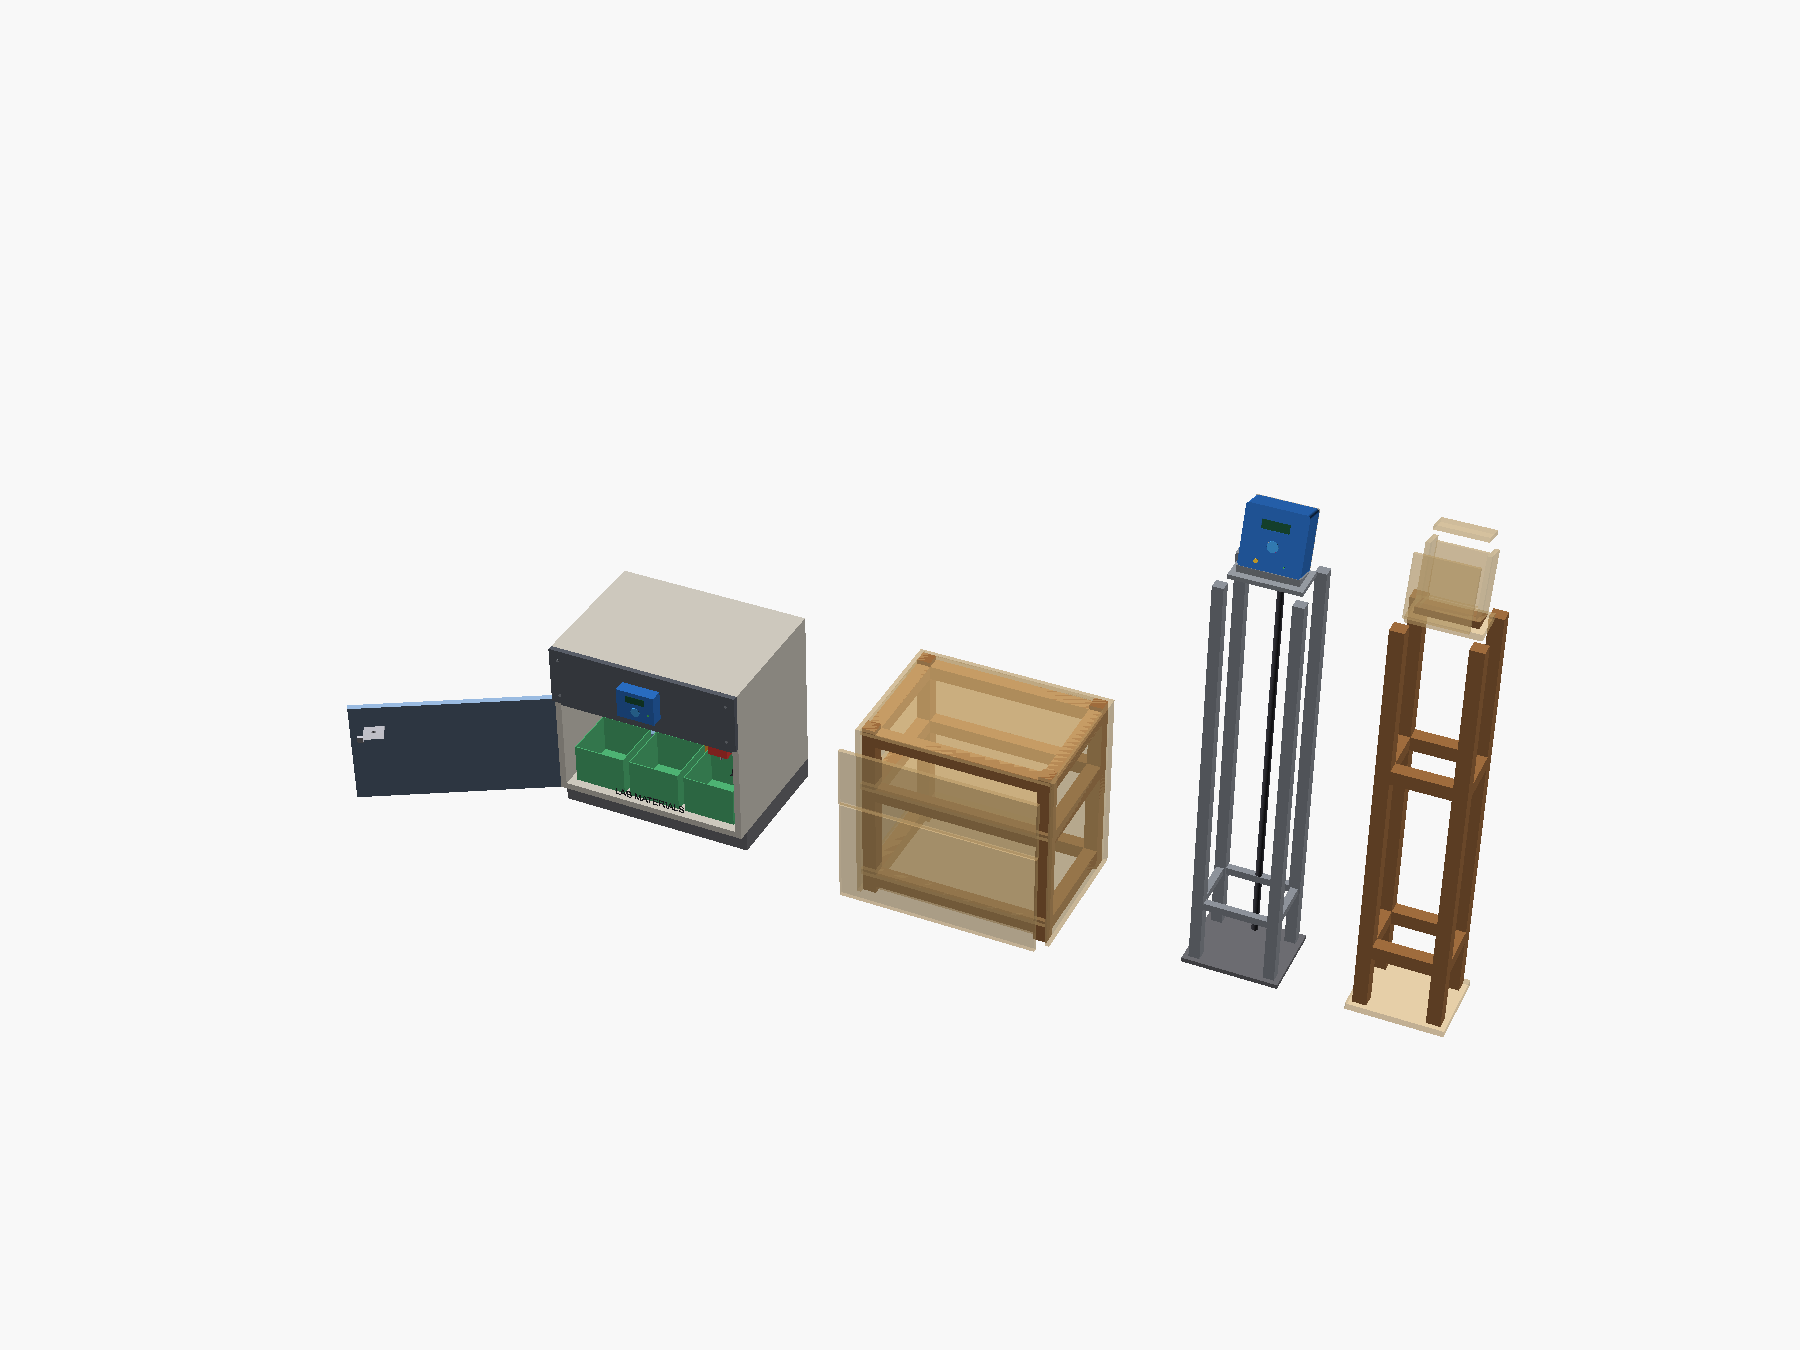
\includegraphics[width=\linewidth, trim=330 290 270 455, clip]{figures/all.png}
\end{figure}

\sectionhead{Hardware Components}

Table~\ref{tab:bom} lists every part used and the job it does. Quantities are per reader unless the entry says otherwise. Nothing on the list is rare or difficult to source, which was deliberate. A part that cannot be replaced from a local shop is a part that ends the project on the day it fails.

\begin{table}[H]
\centering
\caption{Parts used and what each one does}
\label{tab:bom}
\begin{tabular}{@{}p{32mm}p{78mm}@{}}
\toprule
Part & What it does \\
\midrule
ESP32 board &
  The small computer. Runs the program and connects to Wi-Fi. One per reader. \\
Fingerprint sensor (R307 or AS608) &
  Reads a finger and checks it against its own stored list. Fingerprints never
  leave it. \\
Small screen (16 by 2) &
  Shows messages. On the cabinet it also shows the one-time code. \\
Relay and 12~V lock &
  The relay is a switch. The lock runs on its own power, not the chip's. \\
Door switch &
  Cabinet only. Tells us if the door really closed. \\
SIM800L text unit &
  Cabinet only. Sends a text when the cabinet opens or someone is refused. \\
Buzzer, light, button &
  The button starts sign-up. The buzzer warns if the door is left open. \\
\bottomrule
\end{tabular}
\end{table}

\sectionhead{Hardware Architecture Design}

The cabinet and the reader box were drawn as 3D models before building. The
cabinet has three shelves behind locked doors. All the electronics sit in a
hidden space behind a screwed panel, so users never see them.

\begin{figure}[H]
\centering
\caption{The cabinet with its service panel removed, showing the electronics bay
above the materials bins}
\label{fig:3d}
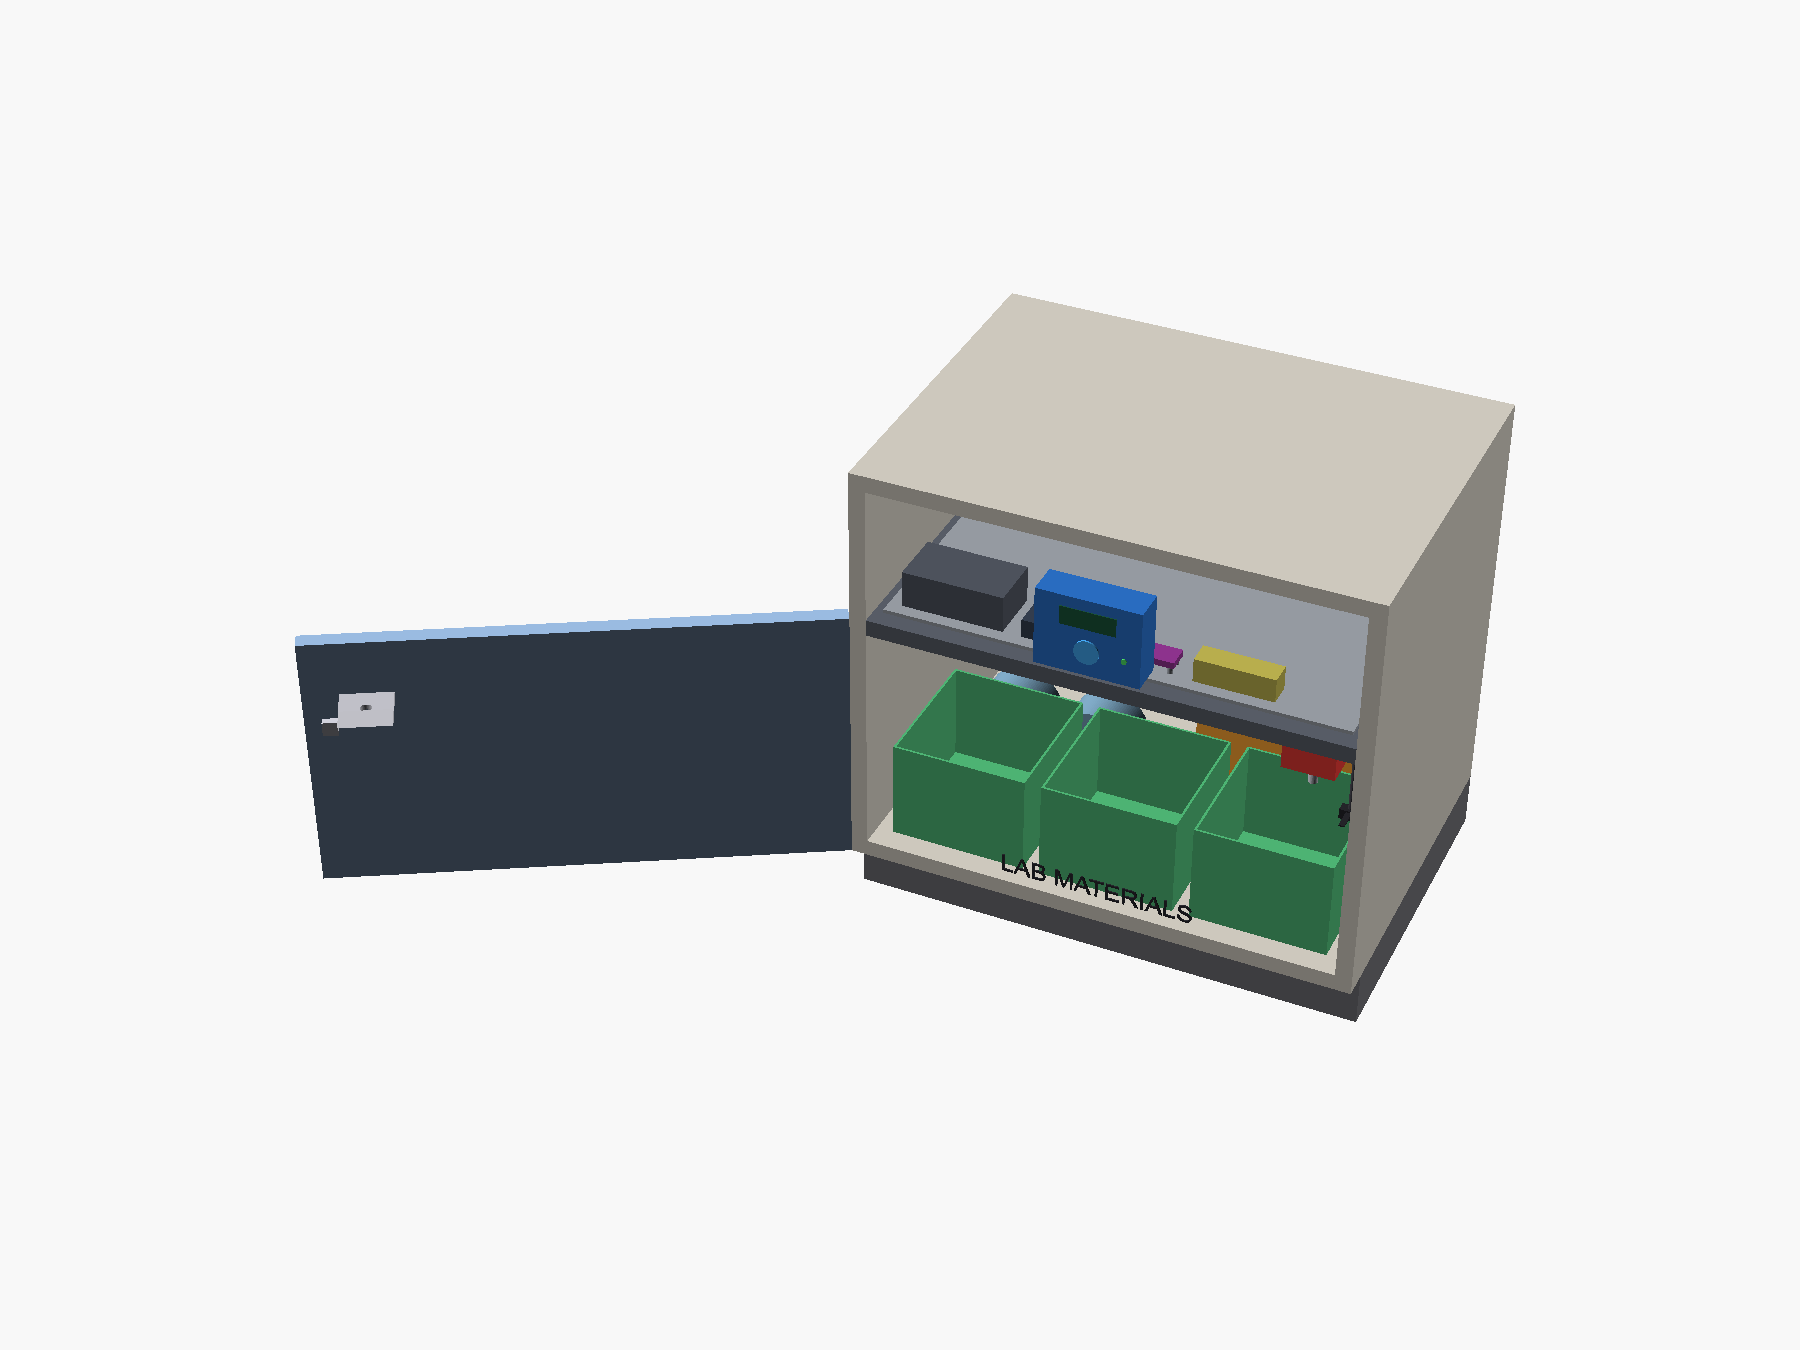
\includegraphics[width=0.92\linewidth]{figures/cabinet_service.png}
\end{figure}

Figure~\ref{fig:head} looks inside the reader box itself, with the back plate
taken off. This is the view used to check that every part fits and to plan the
wiring before anything was cut.

\begin{figure}[H]
\centering
\caption{Inside the reader box with the back plate removed, showing the board,
sensor, relay and lock wiring}
\label{fig:head}
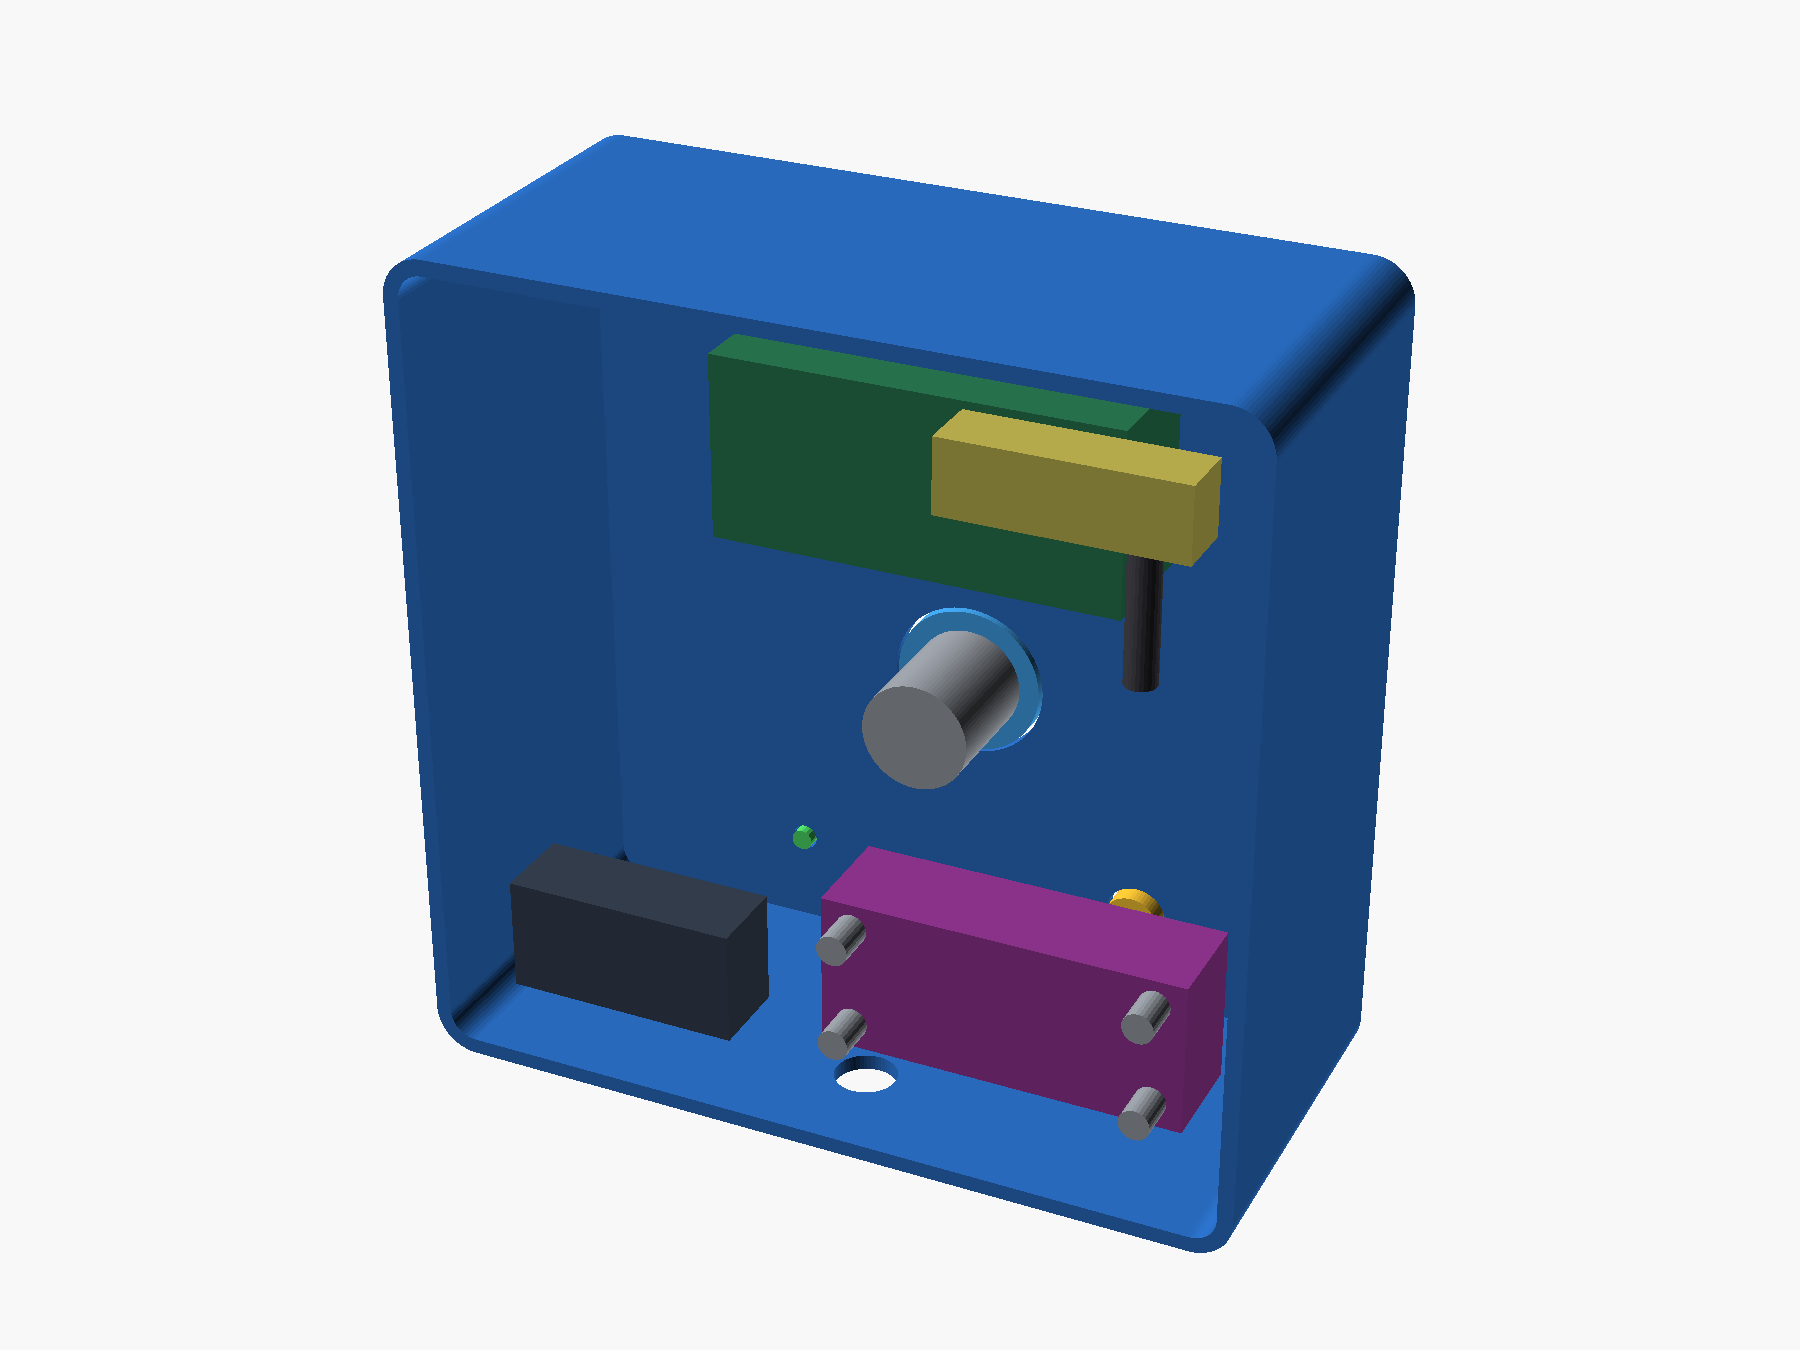
\includegraphics[width=0.82\linewidth]{figures/head_open.png}
\end{figure}

Wiring follows Table~\ref{tab:io}. Three rules guide the layout. First, the lock
gets its own power supply, because it pulls a lot of current when it opens and
would otherwise restart the chip. Second, the text unit also gets its own
supply, for the same reason. Third, one wire on the text unit needs a voltage
reducer, because the chip's signal is too strong for it.

\sectionhead{Data Flow}

Data passes through three programs on its way from a finger to the record: the
firmware on the ESP32 readers, the backend server, and the frontend website.
This section first lists the steps of one complete use, then follows the data
through each program in turn, with a flowchart for each. It ends one level
lower, with the instructions the chip itself executes.

\subsectionhead{Steps in One Complete Use}

The sequence below traces one successful use from beginning to end, from the
first finger at the door to the borrowed items appearing in the record. It is
the same path drawn in Figure~\ref{fig:overall}.

\begin{enumerate}
  \item Someone puts a finger on the door sensor. The sensor finds a match and
        gives back a slot number.
  \item The door reader sends that number, plus its own ID and password, to the
        server.
  \item The server looks up the person, starts a 120-second session, saves the
        record, and replies ``allowed''.
  \item The door reader opens the lock for 3 seconds and shows a message.
  \item Someone puts a finger on the cabinet sensor. The cabinet reader sends
        its own request.
  \item The server checks whether this is the same person who has the running
        session. If yes, it makes a one-time code and saves the record. If no,
        it refuses and saves that too.
  \item The cabinet releases its lock for 4 seconds and shows the code. The
        server queues a text message, which the cabinet sends on its next check.
        If the door is left open, the buzzer sounds.
  \item The person types the code and the borrowed items into the website. The
        server accepts it only if the code is still valid.
\end{enumerate}

\subsectionhead{The ESP32 Firmware}

Each reader runs one program that starts once and then repeats a single loop for
as long as it has power. Figure~\ref{fig:firmware} shows the cabinet reader,
which has the most to do. The door reader runs the same loop without the door
switch and the text messages. The only way out of the program is at start-up:
a reader whose fingerprint sensor does not answer shows an error and stops
there, since it has no work to do without one.

\begin{figure}[H]
\centering
\caption{The cabinet reader's firmware: start-up, then one pass of the loop}
\label{fig:firmware}
\begin{tikzpicture}[flow, x=1mm, y=0.93mm,
  proc/.append style={text width=24mm, minimum width=26mm},
  io/.append style={text width=19mm},
  end/.style = {term, minimum width=14mm}]

\node[term] (on)   at (0,0)    {Start};
\node[proc] (su1)  at (0,-12)  {Start serial, screen\\and lock};
\node[dec]  (sen)  at (0,-27)  {Sensor\\found?};
\node[deny] (hlt)  at (34,-27) {Show error\\and halt};
\node[end]  (x1)   at (62,-27) {Stop};
\node[proc] (su2)  at (0,-43)  {Join Wi-Fi, set clock,\\start SIM800L};
\node[proc] (mem)  at (0,-57)  {Check free memory};
\node[dec]  (door) at (0,-72)  {Door switch\\changed?};
\node[proc] (buzz) at (34,-72) {Warn at 30~s,\\alarm at 60~s};
\node[dec]  (btn)  at (0,-90)  {Enroll button\\pressed?};
\node[proc] (enr)  at (34,-90) {Run one\\enrollment step};
\node[io]   (poll) at (0,-106) {Poll sensor\\on UART2};
\node[dec]  (fp)   at (0,-121) {Finger\\matched?};
\node[io]   (scan) at (34,-121) {Send\\cabinet:slot};
\node[dec]  (ok)   at (68,-121) {Reply is\\unlock?};
\node[proc] (open) at (102,-137) {Release lock 4~s,\\show code 15~s};
\node[deny] (why)  at (68,-137) {Show the reason,\\stay locked};
\node[dec]  (hb)   at (0,-155) {30~s since\\heartbeat?};
\node[io]   (hbs)  at (34,-155) {Send\\heartbeat};
\node[dec]  (sms)  at (0,-173) {15~s since\\SMS check?};
\node[io]   (smss) at (34,-173) {Send up to 3\\queued texts};
\node[proc] (wait) at (0,-190) {Wait 50 ms};

\draw[arr] (on.south) -- (su1.north);
\draw[arr] (su1.south) -- (sen.north);
\draw[arr] (sen.east) -- node[lbl, above] {no} (hlt.west);
\draw[arr] (hlt.east) -- (x1.west);
\draw[arr] (sen.south) -- node[lbl, left, pos=0.3] {yes} (su2.north);
\draw[arr] (su2.south) -- (mem.north);
\draw[arr] (mem.south) -- (door.north);
\draw[arr] (door.east) -- node[lbl, above] {yes} (buzz.west);
\draw[arr] (door.south) -- node[lbl, left, pos=0.15] {no} (btn.north);
\draw[arr] (buzz.south) |- (0,-81);
\draw[arr] (btn.east) -- node[lbl, above] {yes} (enr.west);
\draw[arr] (enr.east) -- (52,-90) |- (mem.east);
\draw[arr] (btn.south) -- node[lbl, left, pos=0.3] {no} (poll.north);
\draw[arr] (poll.south) -- (fp.north);
\draw[arr] (fp.east) -- node[lbl, above] {yes} (scan.west);
\draw[arr] (scan.east) -- (ok.west);
\draw[arr] (ok.east) -| node[lbl, above, pos=0.25] {yes} (open.north);
\draw[arr] (ok.south) -- node[lbl, right] {no} (why.north);
\draw[arr] (open.south) |- (0,-146);
\draw (why.south) -- (68,-146);
\draw[arr] (fp.south) -- node[lbl, left, pos=0.1] {no} (hb.north);
\draw[arr] (hb.east) -- node[lbl, above] {yes} (hbs.west);
\draw[arr] (hbs.south) |- (0,-164);
\draw[arr] (hb.south) -- node[lbl, left, pos=0.15] {no} (sms.north);
\draw[arr] (sms.east) -- node[lbl, above] {yes} (smss.west);
\draw[arr] (smss.south) |- (0,-182);
\draw[arr] (sms.south) -- node[lbl, left, pos=0.15] {no} (wait.north);
\draw[arr] (wait.west) -- (-20,-190) |- node[lbl, left, pos=0.25, rotate=90, anchor=south] {repeat forever} (mem.west);

\end{tikzpicture}

\end{figure}

Each pass of the loop asks a fixed list of questions in the same order: has the
door switch changed, was the enroll button pressed, is there a finger on the
sensor, is a heartbeat due, and are text messages due. Most passes answer no to
all of them and end with a 50 ms wait, so the loop runs about twenty times a
second. The timers are kept by comparing the chip's millisecond clock against
the last time each job ran, rather than by stopping to wait for them.

Two steps do stop the loop while they run: holding the lock open for 4 seconds,
and holding a message on the screen. During those moments the reader cannot take
another finger. The Wi-Fi connection is not affected, because the Wi-Fi stack
runs on the chip's other core.

\subsectionhead{The Backend}

Every scan from either reader arrives at the same address on the server, and
Figure~\ref{fig:backend} shows what the server does with it. The first two
checks apply to both readers: the request must come from a known reader with
the right secret, and the finger must belong to a registered person. After that
the path splits by which reader sent the scan.

\begin{figure}[H]
\centering
\caption{How the backend decides a scan from the door or the cabinet}
\label{fig:backend}
\begin{tikzpicture}[flow, x=1mm, y=1mm,
  side/.style = {deny, text width=19mm, minimum width=21mm},
  end/.style = {term, minimum width=14mm}]

\node[term] (in)   at (51,0)    {Start};
\node[io]   (rcv)  at (51,-13)  {Receive scan\\request};
\node[proc] (auth) at (51,-27)  {Read reader ID\\and secret headers};
\node[dec]  (dev)  at (51,-43)  {Known and\\active reader?};
\node[side] (401)  at (88,-43)  {Reply 401,\\nothing saved};
\node[end]  (x1)   at (113,-43) {Stop};
\node[dec]  (tok)  at (51,-61)  {Finger bound\\to a user?};
\node[side] (unr)  at (88,-61)  {Save refusal:\\unregistered};
\node[end]  (x2)   at (113,-61) {Stop};
\node[dec]  (kind) at (51,-79)  {Door or\\cabinet?};

\node[dec]  (act)  at (24,-97)  {Account\\active?};
\node[side] (ina)  at (-7,-97)  {Save refusal:\\account inactive};
\node[end]  (x3)   at (-7,-110) {Stop};
\node[proc] (sess) at (24,-115) {Open or extend\\session to now + 120~s};
\node[proc] (dg)   at (24,-130) {Save door grant};
\node[proc] (du)   at (24,-143) {Reply unlock};
\node[end]  (x4)   at (24,-155) {Stop};

\node[dec]  (has)  at (78,-97)  {Open session\\for this user?};
\node[side] (tail) at (109,-97) {Save refusal:\\no session\\(tailgating)};
\node[end]  (x5)   at (109,-111) {Stop};
\node[dec]  (live) at (78,-122) {Session not\\yet expired?};
\node[side] (exp)  at (109,-122) {Close it, save\\refusal: expired};
\node[end]  (x6)   at (109,-135) {Stop};
\node[proc] (code) at (78,-140) {Issue 6-character\\code, valid 15 min};
\node[proc] (bg)   at (78,-154) {Save cabinet grant};
\node[proc] (bu)   at (78,-167) {Reply unlock\\with the code};
\node[end]  (x7)   at (78,-180) {Stop};

\draw[arr] (in.south) -- (rcv.north);
\draw[arr] (rcv.south) -- (auth.north);
\draw[arr] (auth.south) -- (dev.north);
\draw[arr] (dev.east) -- node[lbl, above] {no} (401.west);
\draw[arr] (401.east) -- (x1.west);
\draw[arr] (dev.south) -- node[lbl, right] {yes} (tok.north);
\draw[arr] (tok.east) -- node[lbl, above] {no} (unr.west);
\draw[arr] (unr.east) -- (x2.west);
\draw[arr] (tok.south) -- node[lbl, right] {yes} (kind.north);
\draw[arr] (kind.west) -| node[lbl, above, pos=0.3] {door} (act.north);
\draw[arr] (kind.east) -| node[lbl, above, pos=0.3] {cabinet} (has.north);

\draw[arr] (act.west) -- node[lbl, above] {no} (ina.east);
\draw[arr] (ina.south) -- (x3.north);
\draw[arr] (act.south) -- node[lbl, right] {yes} (sess.north);
\draw[arr] (sess.south) -- (dg.north);
\draw[arr] (dg.south) -- (du.north);
\draw[arr] (du.south) -- (x4.north);

\draw[arr] (has.east) -- node[lbl, above] {no} (tail.west);
\draw[arr] (tail.south) -- (x5.north);
\draw[arr] (has.south) -- node[lbl, right] {yes} (live.north);
\draw[arr] (live.east) -- node[lbl, above] {no} (exp.west);
\draw[arr] (exp.south) -- (x6.north);
\draw[arr] (live.south) -- node[lbl, right] {yes} (code.north);
\draw[arr] (code.south) -- (bg.north);
\draw[arr] (bg.south) -- (bu.north);
\draw[arr] (bu.south) -- (x7.north);

\end{tikzpicture}

\end{figure}

A door scan only has to confirm that the account is active, then opens a
session that ends 120 seconds later. A cabinet scan has to find an open session
belonging to the same person. There is no separate ``wrong person'' check,
because the server looks sessions up by the person who just scanned. If someone
else opened the door, the person at the cabinet simply has no session, and the
refusal is recorded as possible tailgating.

Every box in the figure that says ``save'' writes one row to the record. The
server has no route that edits or deletes those rows. Each new row is also
pushed straight to any dashboard that is open, and, if it is an opening or a
refusal, a text message is queued for the people subscribed to that alert.

\subsectionhead{The Frontend}

The website never talks to a reader. Everything it shows comes from the backend,
and everything a person types goes back to it. Figure~\ref{fig:frontend} shows
the checkout page, which is where the cabinet's one-time code is used.

\begin{figure}[H]
\centering
\caption{The checkout page, from opening it to the record being saved}
\label{fig:frontend}
\begin{tikzpicture}[flow, x=1mm, y=1mm,
  end/.style = {term, minimum width=14mm}]

\node[term] (st)   at (0,0)    {Start};
\node[proc] (open) at (0,-12)  {Open the\\checkout page};
\node[dec]  (auth) at (0,-27)  {Signed in?};
\node[proc] (lgn)  at (38,-27) {Go to the\\sign-in page};
\node[end]  (x1)   at (66,-27) {Stop};
\node[proc] (ask)  at (0,-44)  {Every 5~s, ask if a\\code is waiting};
\node[dec]  (wait) at (0,-60)  {Code\\waiting?};
\node[deny] (none) at (38,-60) {Say the cabinet has\\not issued a code};
\node[io]   (type) at (0,-77)  {Type items\\and the code};
\node[io]   (post) at (0,-92)  {Submit to\\/checkouts};
\node[dec]  (chk)  at (0,-109) {Code valid\\for this user?};
\node[deny] (bad)  at (38,-109) {Log rejected code,\\show the error};
\node[proc] (save) at (0,-127) {Save checkout,\\mark code spent};
\node[end]  (x2)   at (0,-140) {Stop};

\draw[arr] (st.south) -- (open.north);
\draw[arr] (open.south) -- (auth.north);
\draw[arr] (auth.east) -- node[lbl, above] {no} (lgn.west);
\draw[arr] (lgn.east) -- (x1.west);
\draw[arr] (auth.south) -- node[lbl, right] {yes} (ask.north);
\draw[arr] (ask.south) -- (wait.north);
\draw[arr] (wait.east) -- node[lbl, above] {no} (none.west);
\draw[arr] (none.north) |- (ask.east);
\draw[arr] (wait.south) -- node[lbl, right] {yes} (type.north);
\draw[arr] (type.south) -- (post.north);
\draw[arr] (post.south) -- (chk.north);
\draw[arr] (chk.east) -- node[lbl, above] {no} (bad.west);
\draw[arr] (bad.north) |- (type.east);
\draw[arr] (chk.south) -- node[lbl, right] {yes} (save.north);
\draw[arr] (save.south) -- (x2.north);

\end{tikzpicture}

\end{figure}

While the page is open it asks the server every 5 seconds whether a code is
waiting. The server answers yes or no and when the code expires, but it never
sends the code itself. The only place the code can be read is the cabinet
screen, so the only way to fill in the form is to have been standing at the
cabinet when it opened. The server checks the code again when the form is sent,
so a code that is guessed, reused, or more than 15 minutes old is refused and
the attempt is recorded.

\subsectionhead{How the Chip Runs the Instructions}

Underneath all of this, the chip repeats one cycle. It fetches an instruction,
works out what it means, and carries it out \parencite{espressif2025}.
Figure~\ref{fig:instruction} shows that cycle. The program itself is stored in
external flash, so an instruction that is not already in the cache has to be
loaded from there first \parencite{espressif2025}.

\begin{figure}[H]
\centering
\caption{The fetch, decode, and execute cycle, with an example of each kind of
instruction from the reader firmware}
\label{fig:instruction}
\begin{tikzpicture}[flow, x=1mm, y=1mm,
  end/.style = {term, minimum width=14mm}]

\node[term] (rst)  at (0,14)   {Start};
\node[proc] (pc)   at (0,0)    {Next address in the\\program counter};
\node[dec]  (hit)  at (0,-17)  {In cache\\or IRAM?};
\node[proc] (fill) at (40,-17) {Cache loads a line\\from external flash};
\node[proc] (fet)  at (0,-35)  {Fetch the instruction};
\node[proc] (dcd)  at (0,-49)  {Decode opcode\\and registers};
\node[dec]  (kind) at (0,-66)  {Kind of\\instruction?};
\node[proc] (alu)  at (-36,-85) {Arithmetic in\\registers (ALU)\\e.g. timer checks};
\node[proc] (ram)  at (0,-85)   {Load or store\\in internal RAM\\e.g. the request};
\node[proc] (per)  at (36,-85)  {Load or store to a\\peripheral register\\e.g. UART2, GPIO 5};
\node[proc] (adv)  at (0,-104)  {Write the result,\\advance the counter};
\node[dec]  (pwr)  at (0,-121)  {Power\\still on?};
\node[end]  (x1)   at (0,-138)  {Stop};

\draw[arr] (rst.south) -- (pc.north);
\draw[arr] (pc.south) -- (hit.north);
\draw[arr] (hit.east) -- node[lbl, above] {no} (fill.west);
\draw[arr] (fill.south) |- (0,-27);
\draw[arr] (hit.south) -- node[lbl, left, pos=0.3] {yes} (fet.north);
\draw[arr] (fet.south) -- (dcd.north);
\draw[arr] (dcd.south) -- (kind.north);
\draw[arr] (kind.west) -| node[lbl, above, pos=0.3] {arithmetic} (alu.north);
\draw[arr] (kind.south) -- node[lbl, right] {memory} (ram.north);
\draw[arr] (kind.east) -| node[lbl, above, pos=0.3] {peripheral} (per.north);
\draw[arr] (alu.south) |- (adv.west);
\draw[arr] (ram.south) -- (adv.north);
\draw[arr] (per.south) |- (adv.east);
\draw[arr] (adv.south) -- (pwr.north);
\draw[arr] (pwr.west) -- node[lbl, above, pos=0.2] {yes} (-56,-121) |- (pc.west);
\draw[arr] (pwr.south) -- node[lbl, right] {no} (x1.north);

\end{tikzpicture}

\end{figure}

Three moments from the firmware show the three kinds of instruction at work.

\textbf{Waiting for the sensor.} Each pass of the loop reads the status of
serial port 2 to see whether the sensor has sent anything. That read is a load
from a peripheral register. Most of the time nothing has arrived, and the loop
moves on.

\textbf{Building the message.} To send a scan, the chip copies text into
internal RAM piece by piece until the request is complete. These are loads and
stores to memory, and this is the step that uses the most of it.

\textbf{Opening the lock.} Releasing the lock is one store to the register that
drives pin 5. The chip then waits 4 seconds and makes one more store to close
it again.

\sectionhead{What a Person Sees at the Reader}

The person standing at the door has one screen and two lines of sixteen
characters to work with. That limit shapes every message: there is no room to
explain, so each line has to say one thing. The wording below is taken from the
firmware exactly as it is displayed.

Table~\ref{tab:lcd-door} lists what the door reader shows. When nothing is
happening it rests on its idle message, so anybody walking up already knows what
to do without being told.

\begin{table}[H]
\centering
\caption{What the door reader displays}
\label{tab:lcd-door}
\linespread{1}\selectfont
\begin{tabular}{@{}p{40mm}p{34mm}p{34mm}@{}}
\toprule
Situation & Top line & Bottom line \\
\midrule
Waiting, nobody inside  & \texttt{Sigurado door}  & \texttt{Scan finger} \\
Waiting, session live   & \texttt{Sigurado door}  & \texttt{session 97s} \\
Asking the server       & \texttt{Checking...}    & \texttt{one moment} \\
Allowed in              & \texttt{Welcome}        & their name \\
Finger not signed up    & \texttt{Not registered} & \texttt{Press enroll} \\
Sensor could not read   & \texttt{Did not read}   & \texttt{please try again} \\
No network              & \texttt{No WiFi yet}    & \texttt{check settings} \\
\bottomrule
\end{tabular}
\end{table}

The second row is worth a note. While a session is running, the idle screen
counts it down in place of the usual prompt, so a person crossing the room can
see how long they have left before the cabinet stops recognising them. The
countdown is a hint rather than the rule: the server holds the real clock, and
the reader only displays what it was last told.

Signing up a finger is a separate sequence, shown in
Table~\ref{tab:lcd-enroll}. The sensor needs the same finger presented more than
once to build a usable template, so the screen walks the person through it one
step at a time.

\begin{table}[H]
\centering
\caption{What the door reader displays while a finger is being signed up}
\label{tab:lcd-enroll}
\linespread{1}\selectfont
\begin{tabular}{@{}p{40mm}p{34mm}p{34mm}@{}}
\toprule
Step & Top line & Bottom line \\
\midrule
First impression  & \texttt{Place finger}   & \texttt{hold still} \\
Lift off          & \texttt{Remove finger}  & \texttt{hold still} \\
Second impression & \texttt{Place again}    & \texttt{hold still} \\
Saving it         & \texttt{Saving...}      & \texttt{one moment} \\
Code to claim it  & the code                & \texttt{Type it on site} \\
Claimed           & \texttt{All set}        & their name \\
Sensor is full    & \texttt{Sensor is full} & \texttt{ask an admin} \\
\bottomrule
\end{tabular}
\end{table}

The code in the fifth row is the reason a template cannot be bound to the wrong
account. The finger belongs to nobody until somebody signs in on the website and
enters that code, so an administrator cannot quietly attach a finger to a person
who never presented it.

The cabinet reader carries the harder messages, because it is the one that says
no. Table~\ref{tab:lcd-cab} shows those. The two refusals are worded
differently on purpose. \texttt{Scan door first} means the person never came
through the door, which is the tailgating case. \texttt{Scan door again} means
they did, but took longer than the session allowed. Telling those apart on the
screen saves the person guessing what went wrong.

\begin{table}[H]
\centering
\caption{What the cabinet reader displays}
\label{tab:lcd-cab}
\linespread{1}\selectfont
\begin{tabular}{@{}p{40mm}p{34mm}p{34mm}@{}}
\toprule
Situation & Top line & Bottom line \\
\midrule
Allowed in            & \texttt{Unlocked}       & their name \\
The one-time code     & \texttt{Your code}      & the code \\
Where to type it      & \texttt{Type it on the} & \texttt{checkout page} \\
Cabinet open          & \texttt{Take what you}  & \texttt{need, then close} \\
No door scan          & \texttt{Still locked}   & \texttt{Scan door first} \\
Session ran out       & \texttt{Still locked}   & \texttt{Scan door again} \\
Door left open        & \texttt{Door is open}   & \texttt{Please close it} \\
Door shut again       & \texttt{Door closed}    & \texttt{Thank you} \\
Text alert going out  & \texttt{Sending alert}  & \texttt{please wait} \\
\bottomrule
\end{tabular}
\end{table}

A refused person is never left without an instruction. Every refusal names the
thing to do next, because a screen that only says no teaches people to rattle
the handle instead.

\sectionhead{The Web Console}

The readers handle the locks. Everything a person reads, types, or checks
happens on the website. It runs in an ordinary browser and talks to the same
server the readers do, so the console never sees a reader directly and cannot
open anything itself.

\subsectionhead{The Public Page}

Figure~\ref{fig:web-landing} shows what a visitor sees before signing in. It
explains the two-scan rule and nothing else. There is no public list of people,
no record of any opening, and no way in except the sign-in link. Accounts are
created by an administrator, so there is no sign-up form to attack.

\begin{figure}[H]
\centering
\caption{The public page, which explains the system without exposing any record}
\label{fig:web-landing}
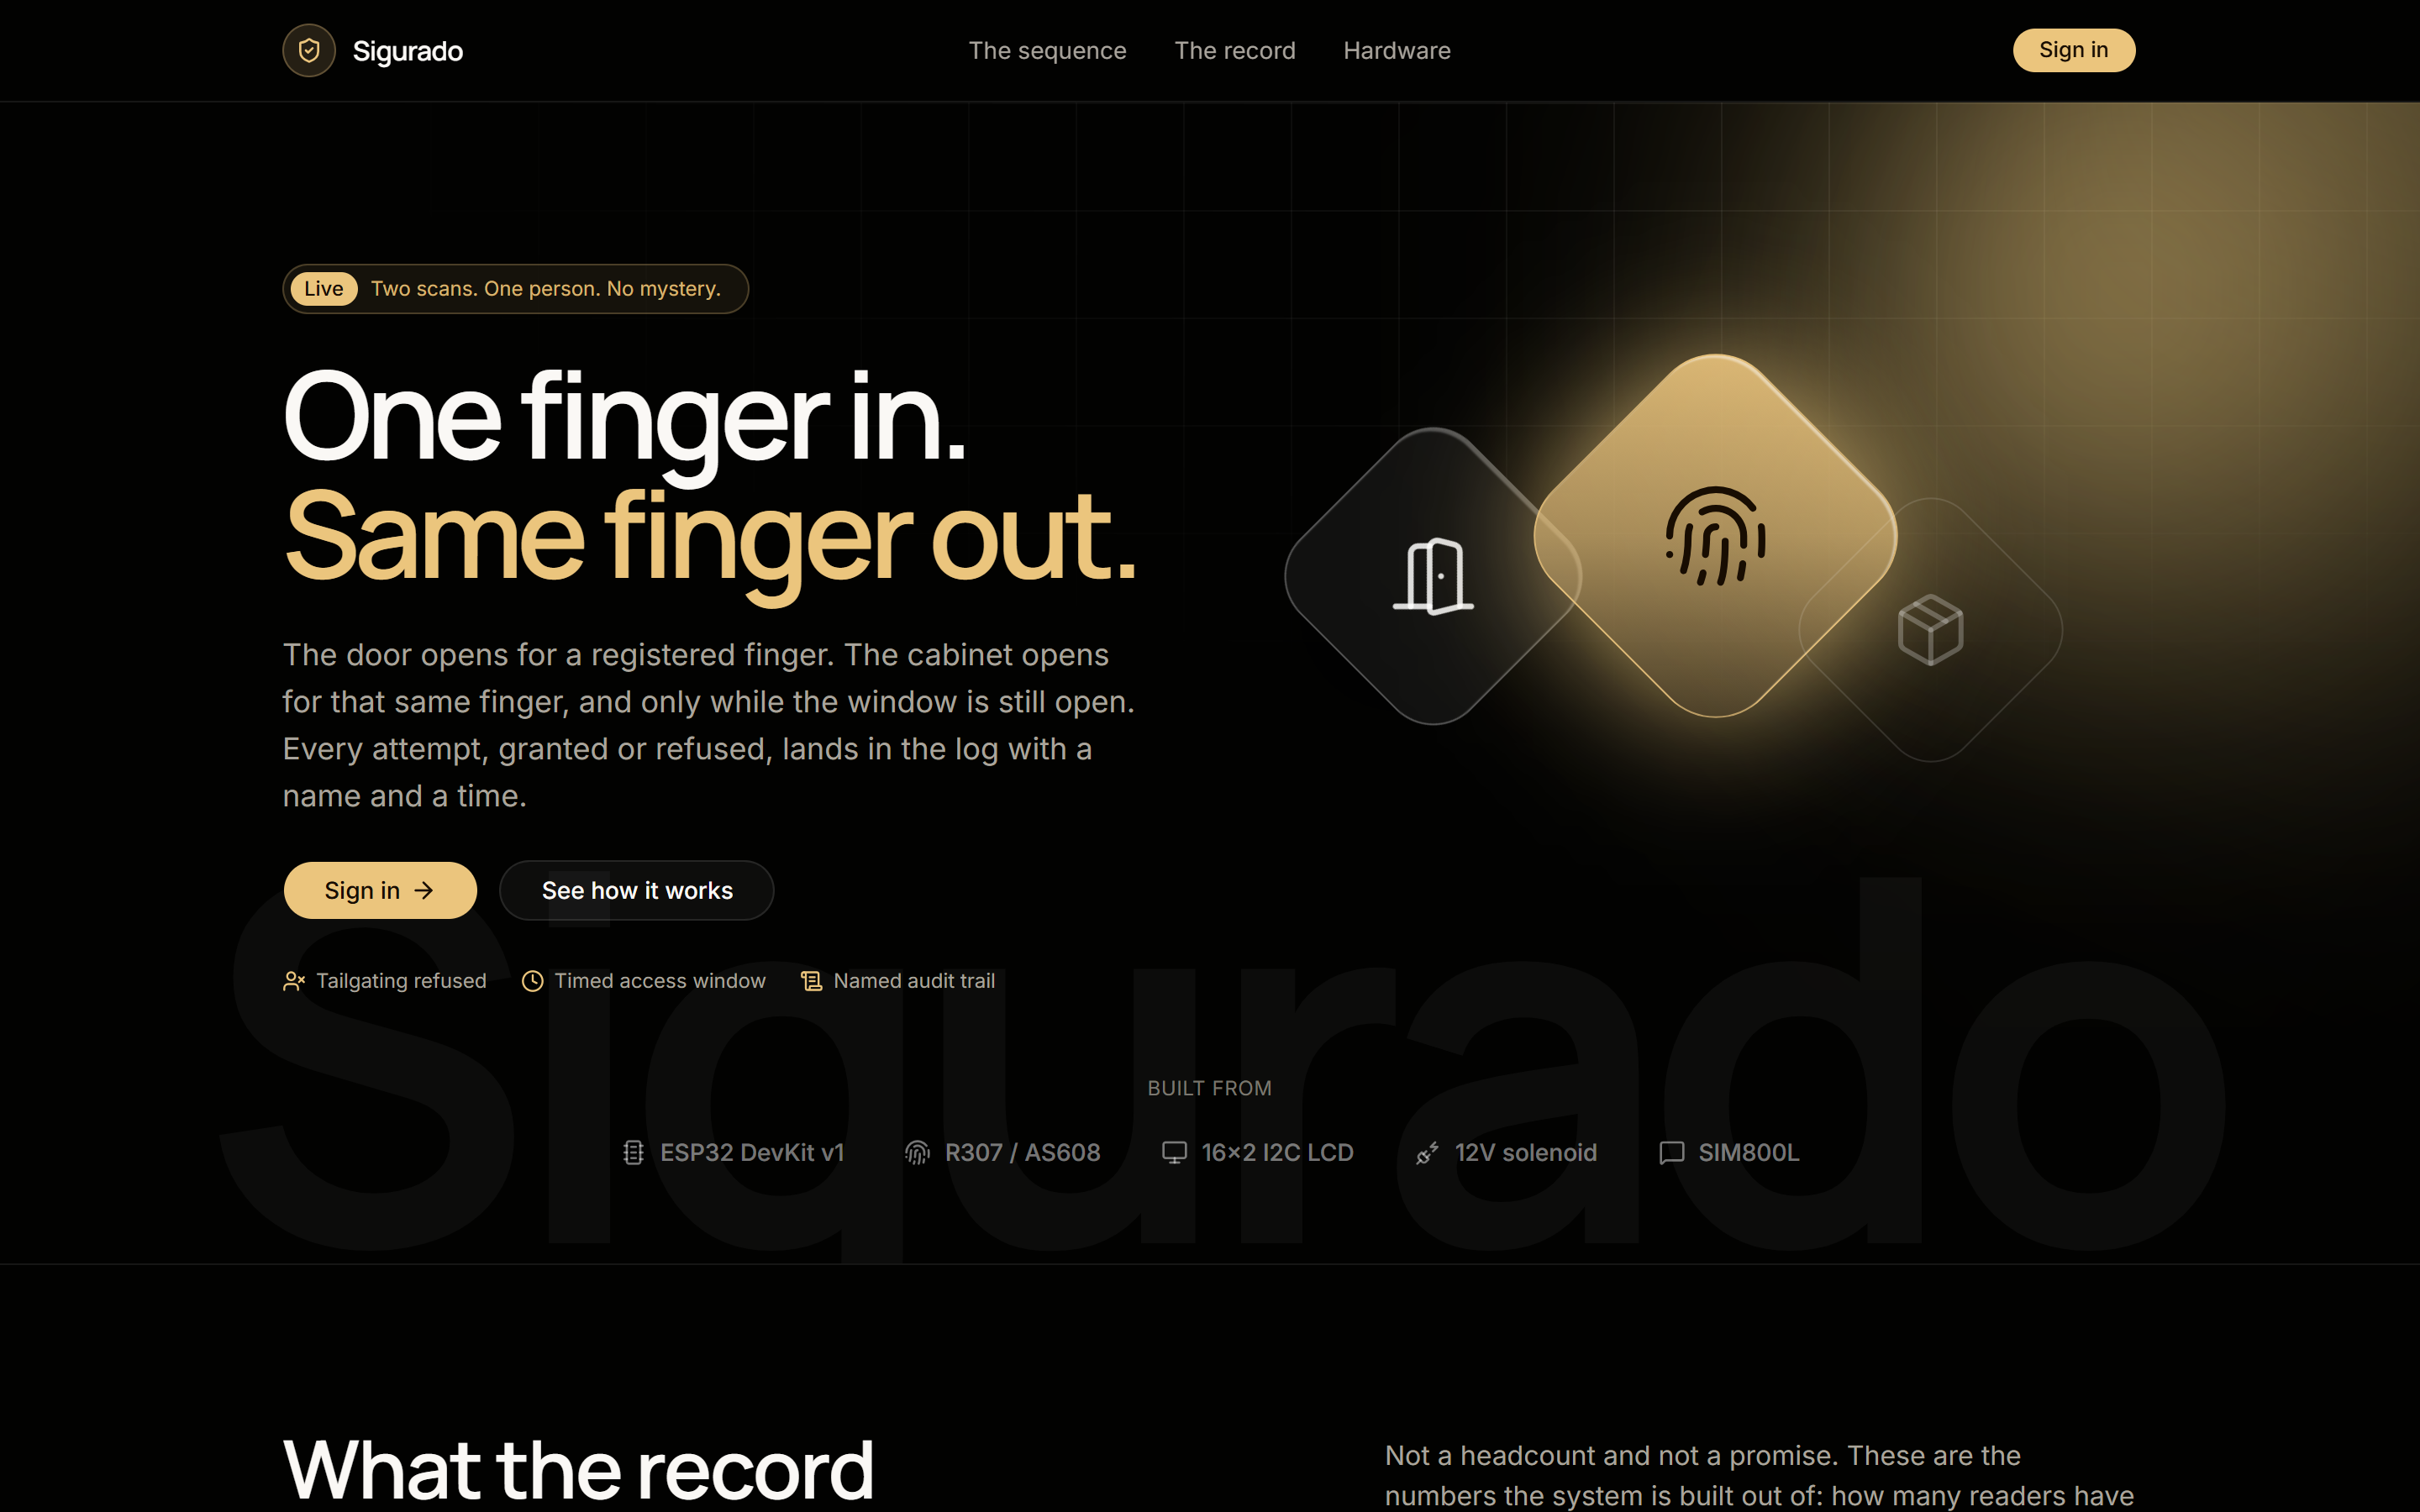
\includegraphics[width=\linewidth]{figures/web-landing.png}
\end{figure}

\subsectionhead{What Each Role Sees}

Signing in decides what the rest of the site shows. A student sees only their
own scans and their own borrowed items. A member of faculty sees everything but
can change nothing. An administrator runs the room: accounts, readers, alerts,
and the stored data. The rule the site enforces is that a student must never see
another student's record, and that nobody at all can edit a reader event.

Figure~\ref{fig:web-dashboard} shows the administrator view. The four counters
along the top answer the question a custodian actually asks on walking in: is
anyone inside the window right now, how many scans have happened today, how many
were refused, and how much was taken. Below them sit the live door sessions,
each with its own countdown, and the stream of decisions as they arrive.

The figure was captured on a quiet morning, so the counters read zero and both
panels are showing their empty state. That is deliberate rather than
unfinished. An empty panel that says only ``no data'' teaches a user nothing, so
each one instead explains what will appear there and when a session or a
decision will cause it. A custodian who has never seen the system before can
therefore read the screen on a quiet day and still understand what it will do on
a busy one.

\begin{figure}[H]
\centering
\caption{The administrator dashboard, showing live sessions and the decisions as
they arrive}
\label{fig:web-dashboard}
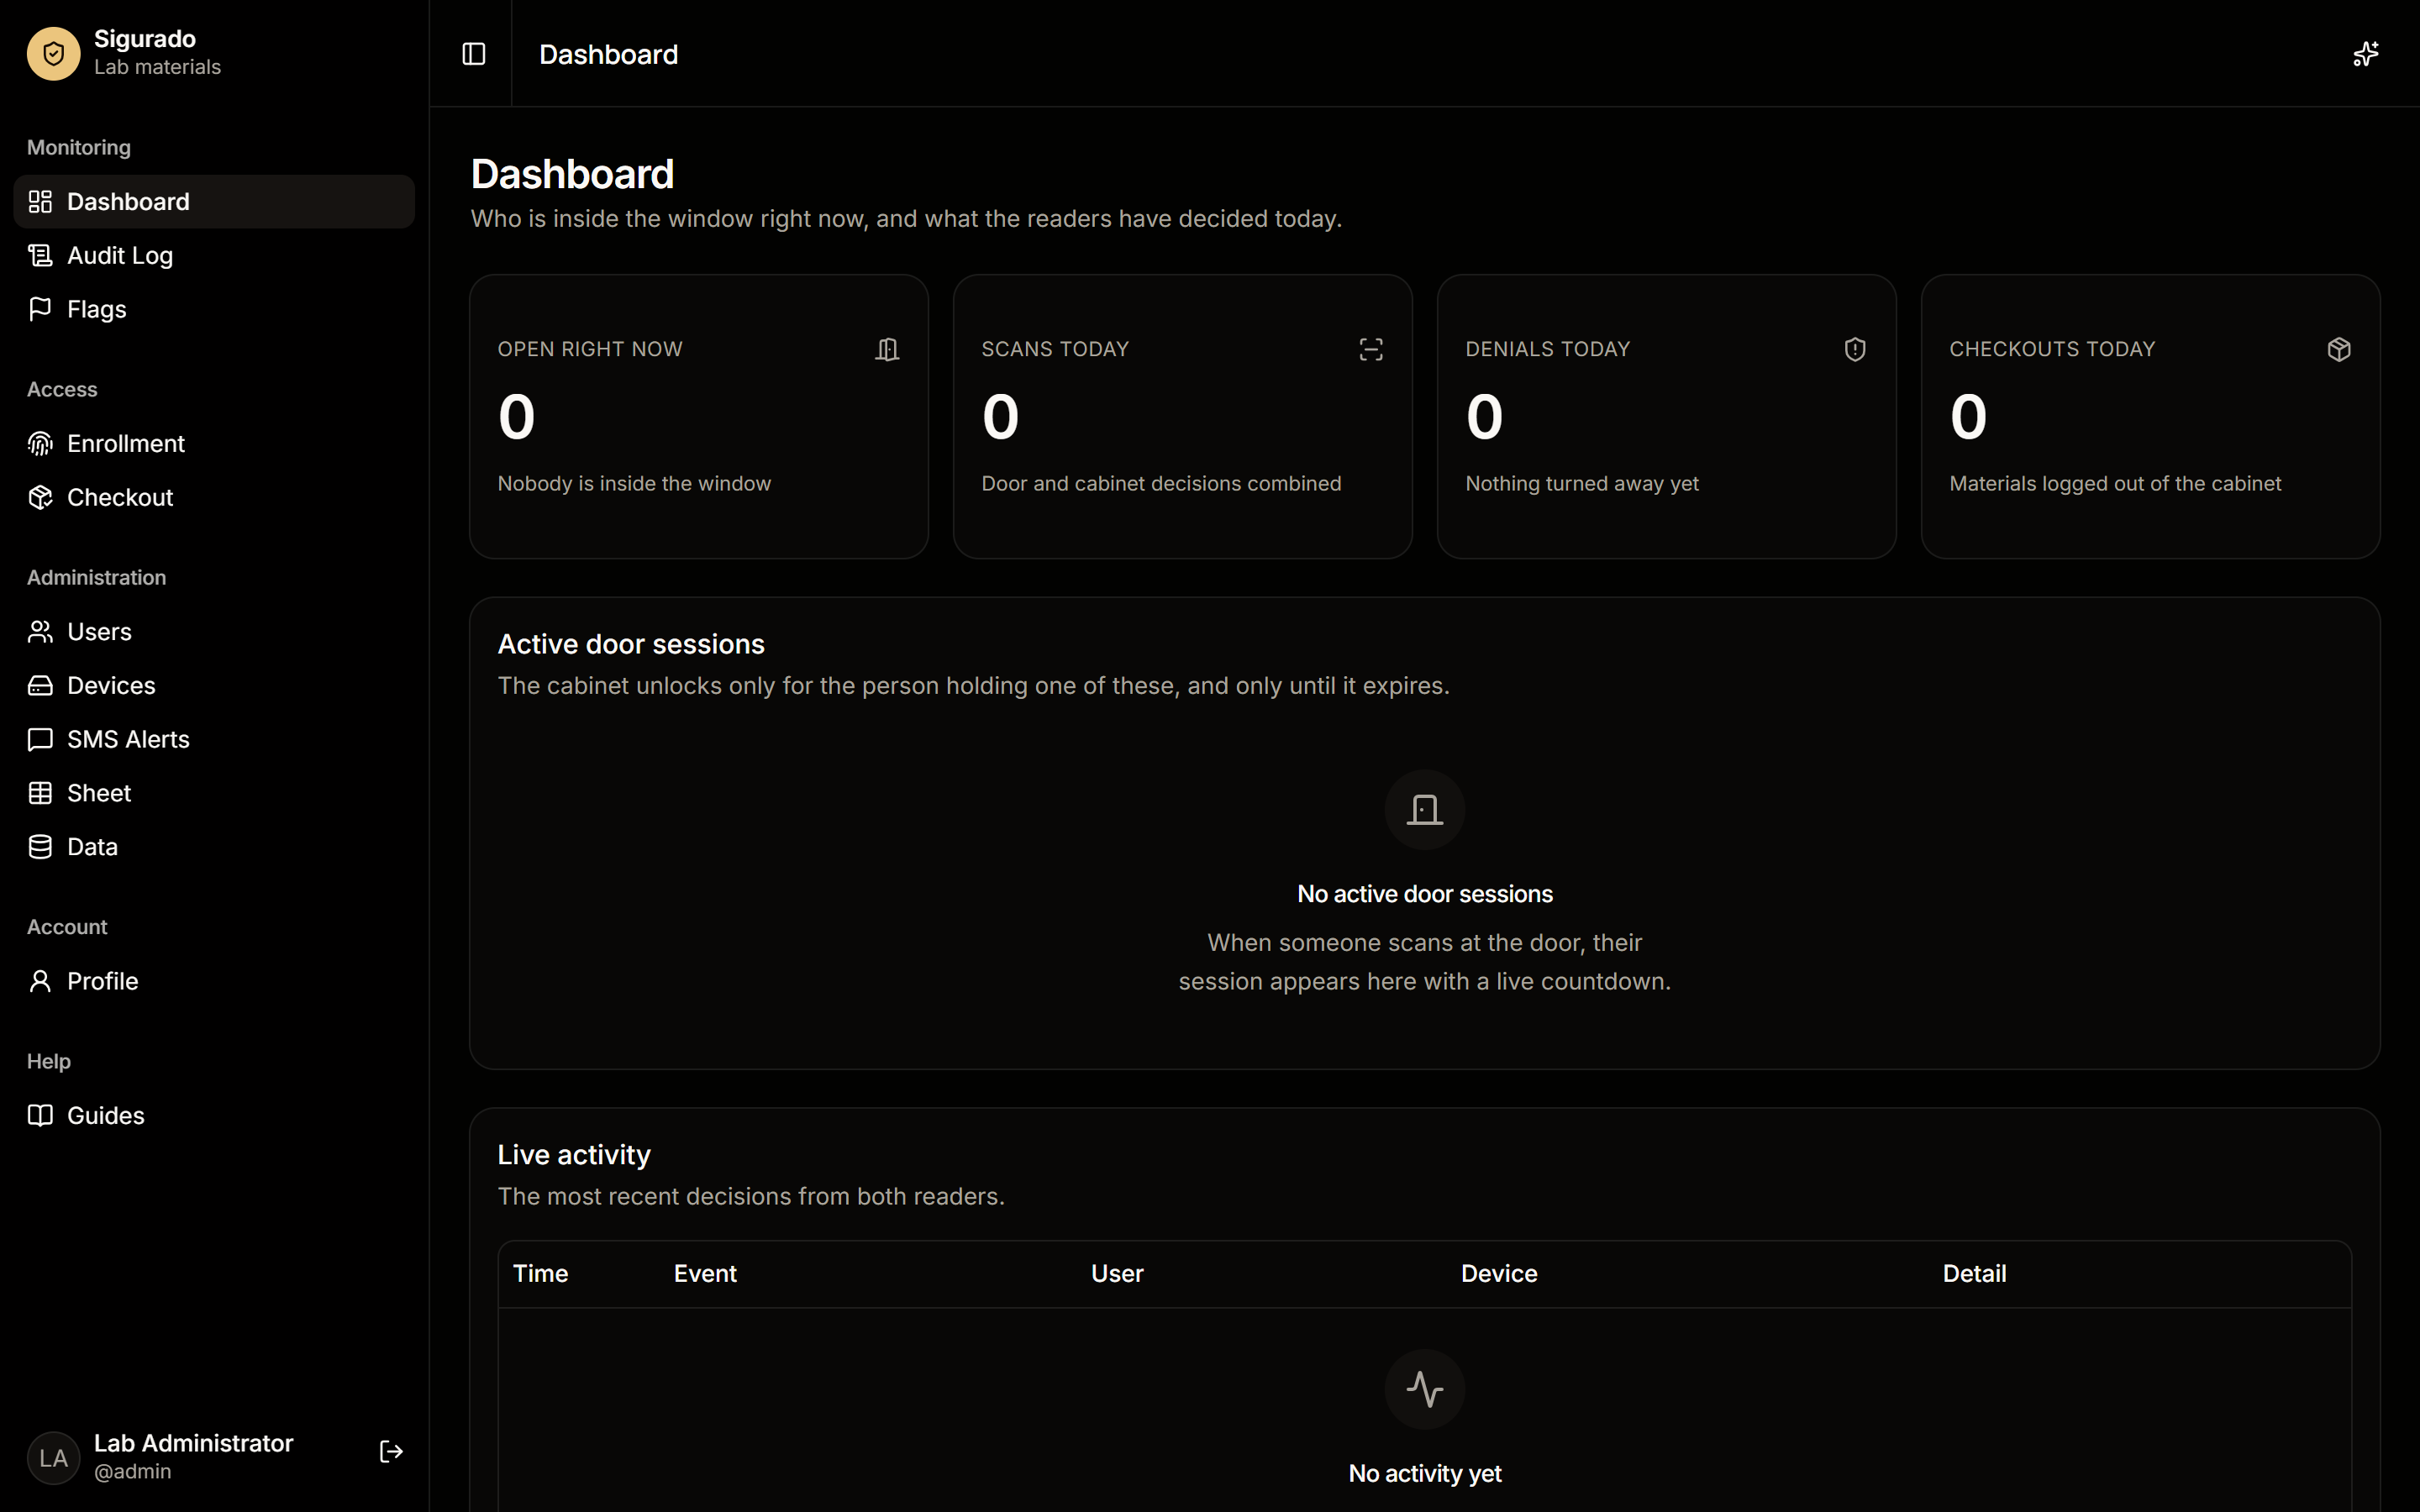
\includegraphics[width=\linewidth]{figures/web-dashboard.png}
\end{figure}

\subsectionhead{The Record}

Figure~\ref{fig:web-sheet} shows the trail as a spreadsheet. Every row is
something a reader reported: a door opened, a cabinet unlocked, a finger
refused, an enrollment code issued. Each carries the time, the person where one
is known, the finger slot, and the reader that saw it. Refusals sit in the same
list as grants, which is what makes a tailgating attempt countable rather than
invisible.

\begin{figure}[H]
\centering
\caption{The trail as a spreadsheet, with grants and refusals in the same list}
\label{fig:web-sheet}
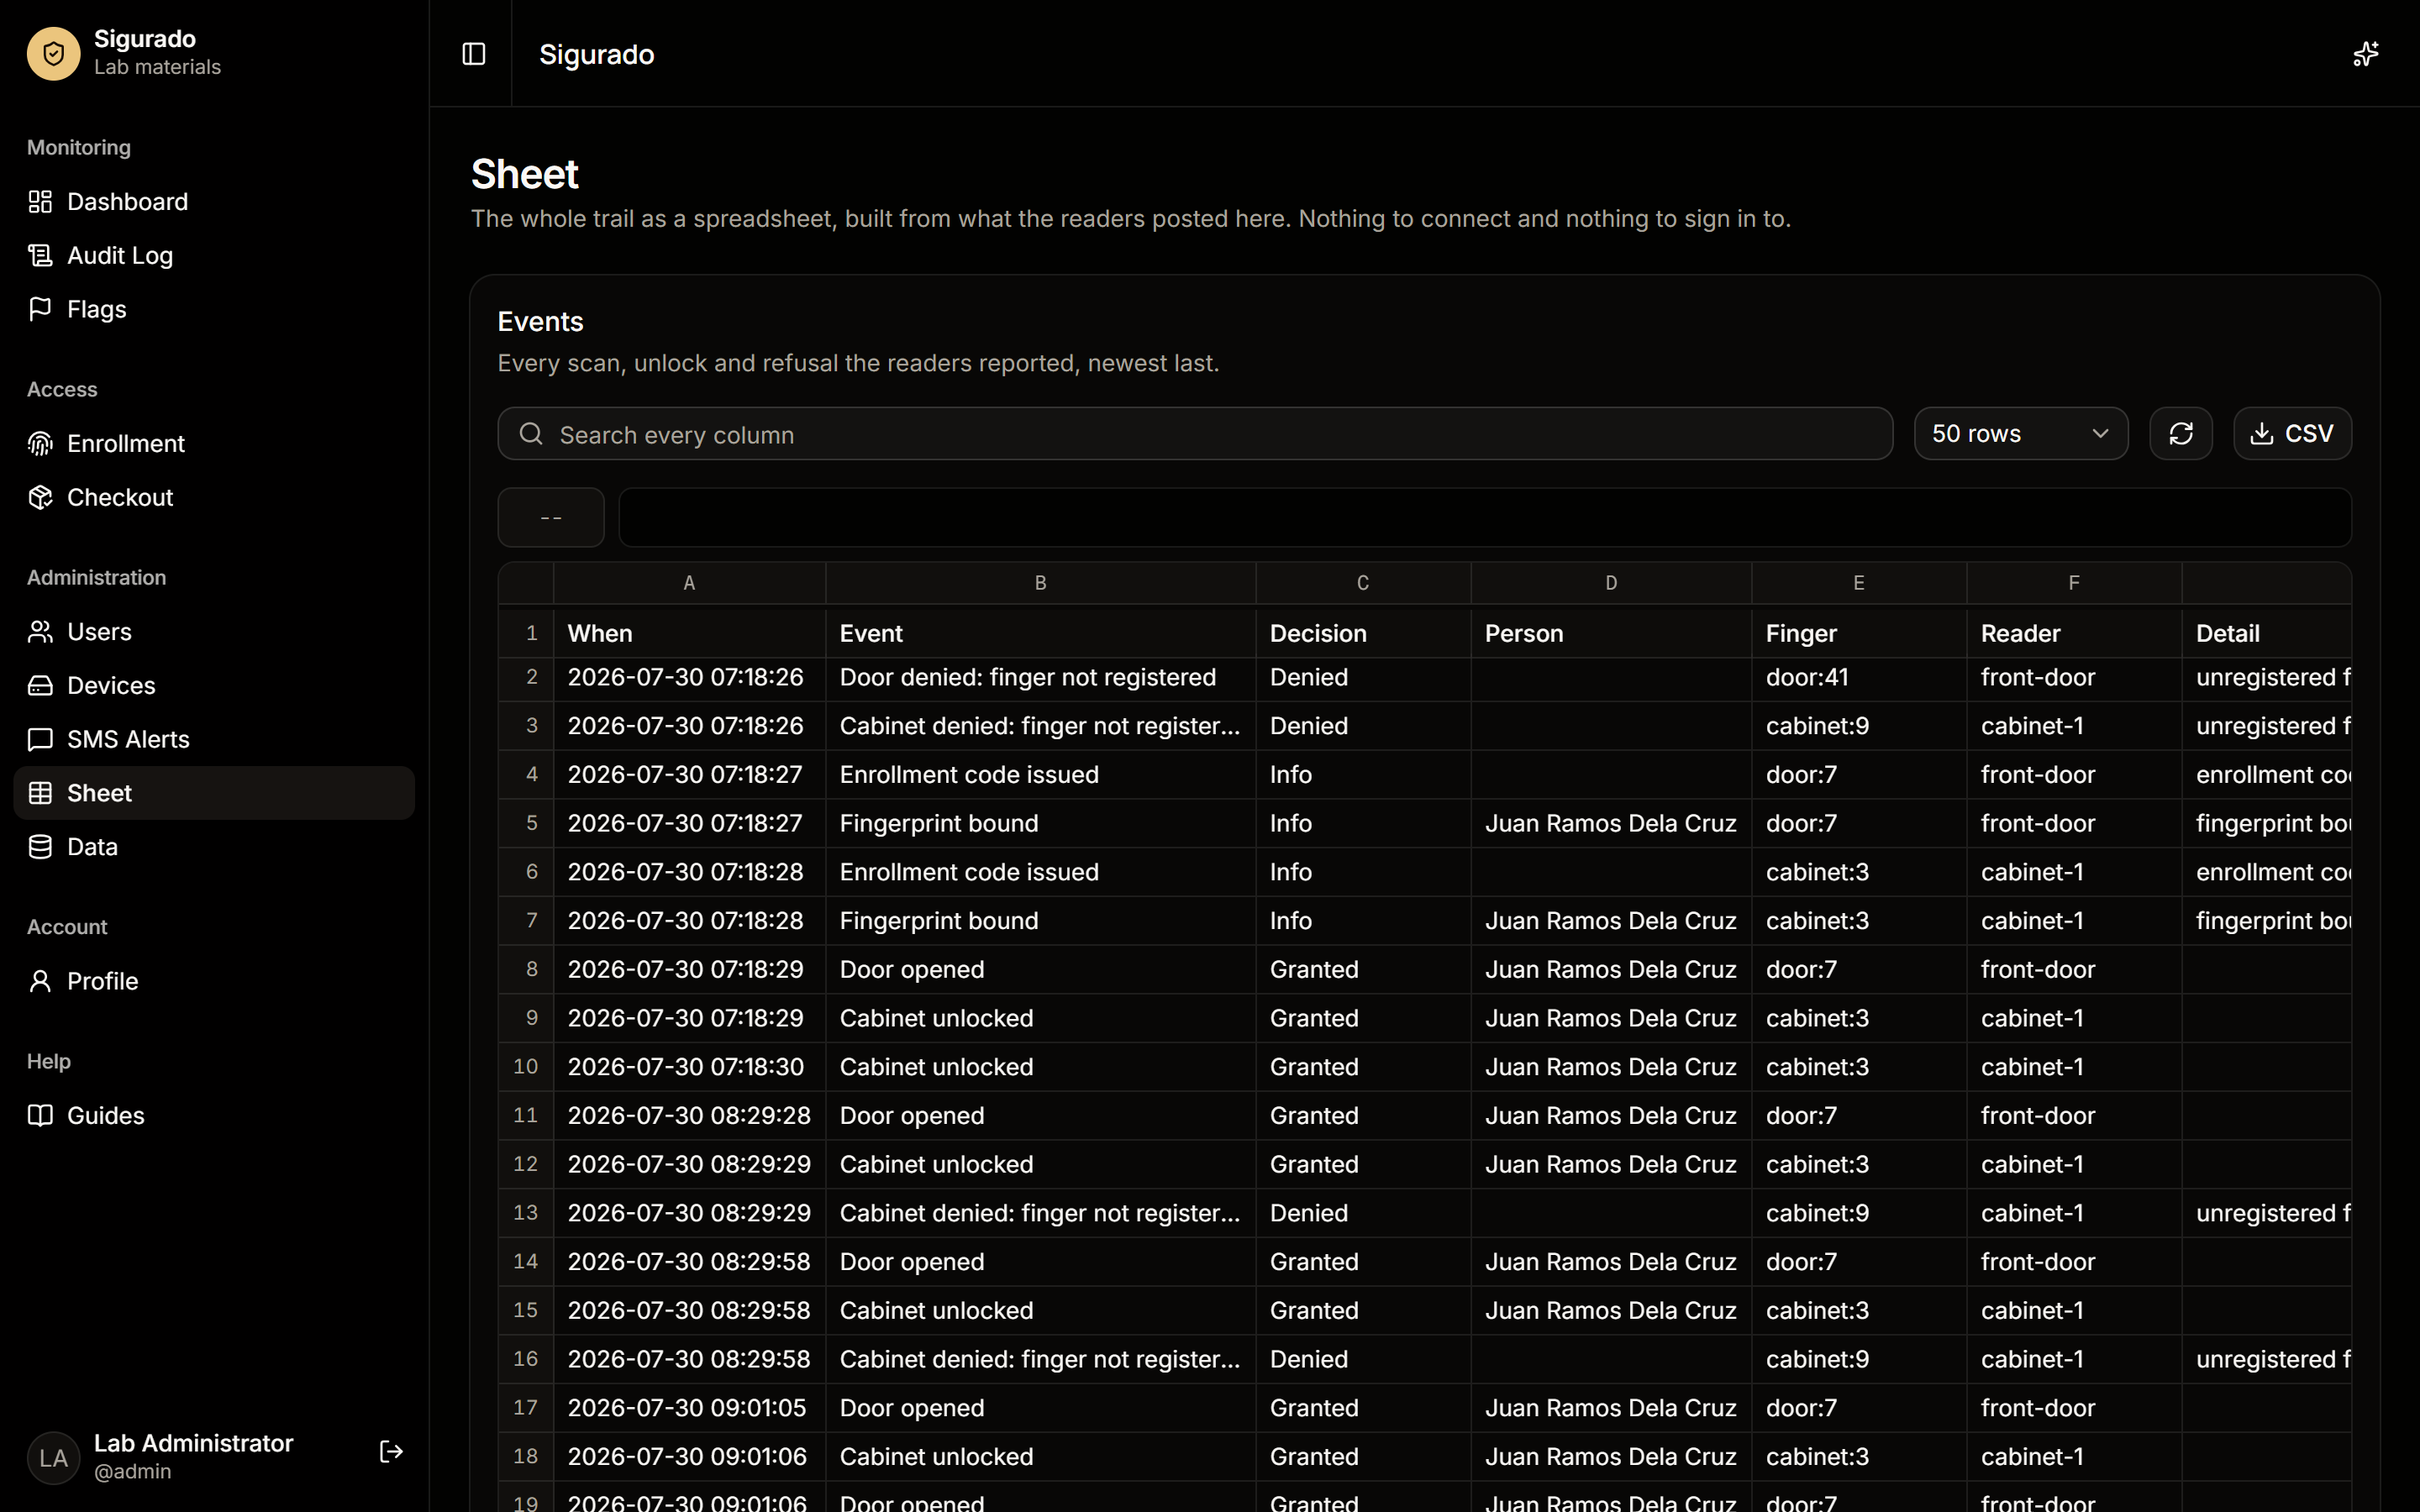
\includegraphics[width=\linewidth]{figures/web-sheet.png}
\end{figure}

The same page exports to CSV, so the record can be kept outside the system as
well. The console also runs eleven checks over the trail and lists whatever does
not add up: an opening with no borrow record behind it, a finger tried
repeatedly and refused, an opening outside laboratory hours, a reader that has
gone quiet. These are the questions a person would have to ask by hand if the
record were on paper.

\subsectionhead{On a Phone}

Most people will reach the site on a phone, standing at the cabinet with the
one-time code still on the screen in front of them. The whole console is built
to work at that size, not just to survive it.
Figure~\ref{fig:web-mobile} shows three of those screens.

\begin{figure}[H]
\centering
\caption{The site on a phone: the public page, the dashboard, and the checkout
form where the one-time code is entered}
\label{fig:web-mobile}
\begin{minipage}[t]{0.31\linewidth}
  \centering
  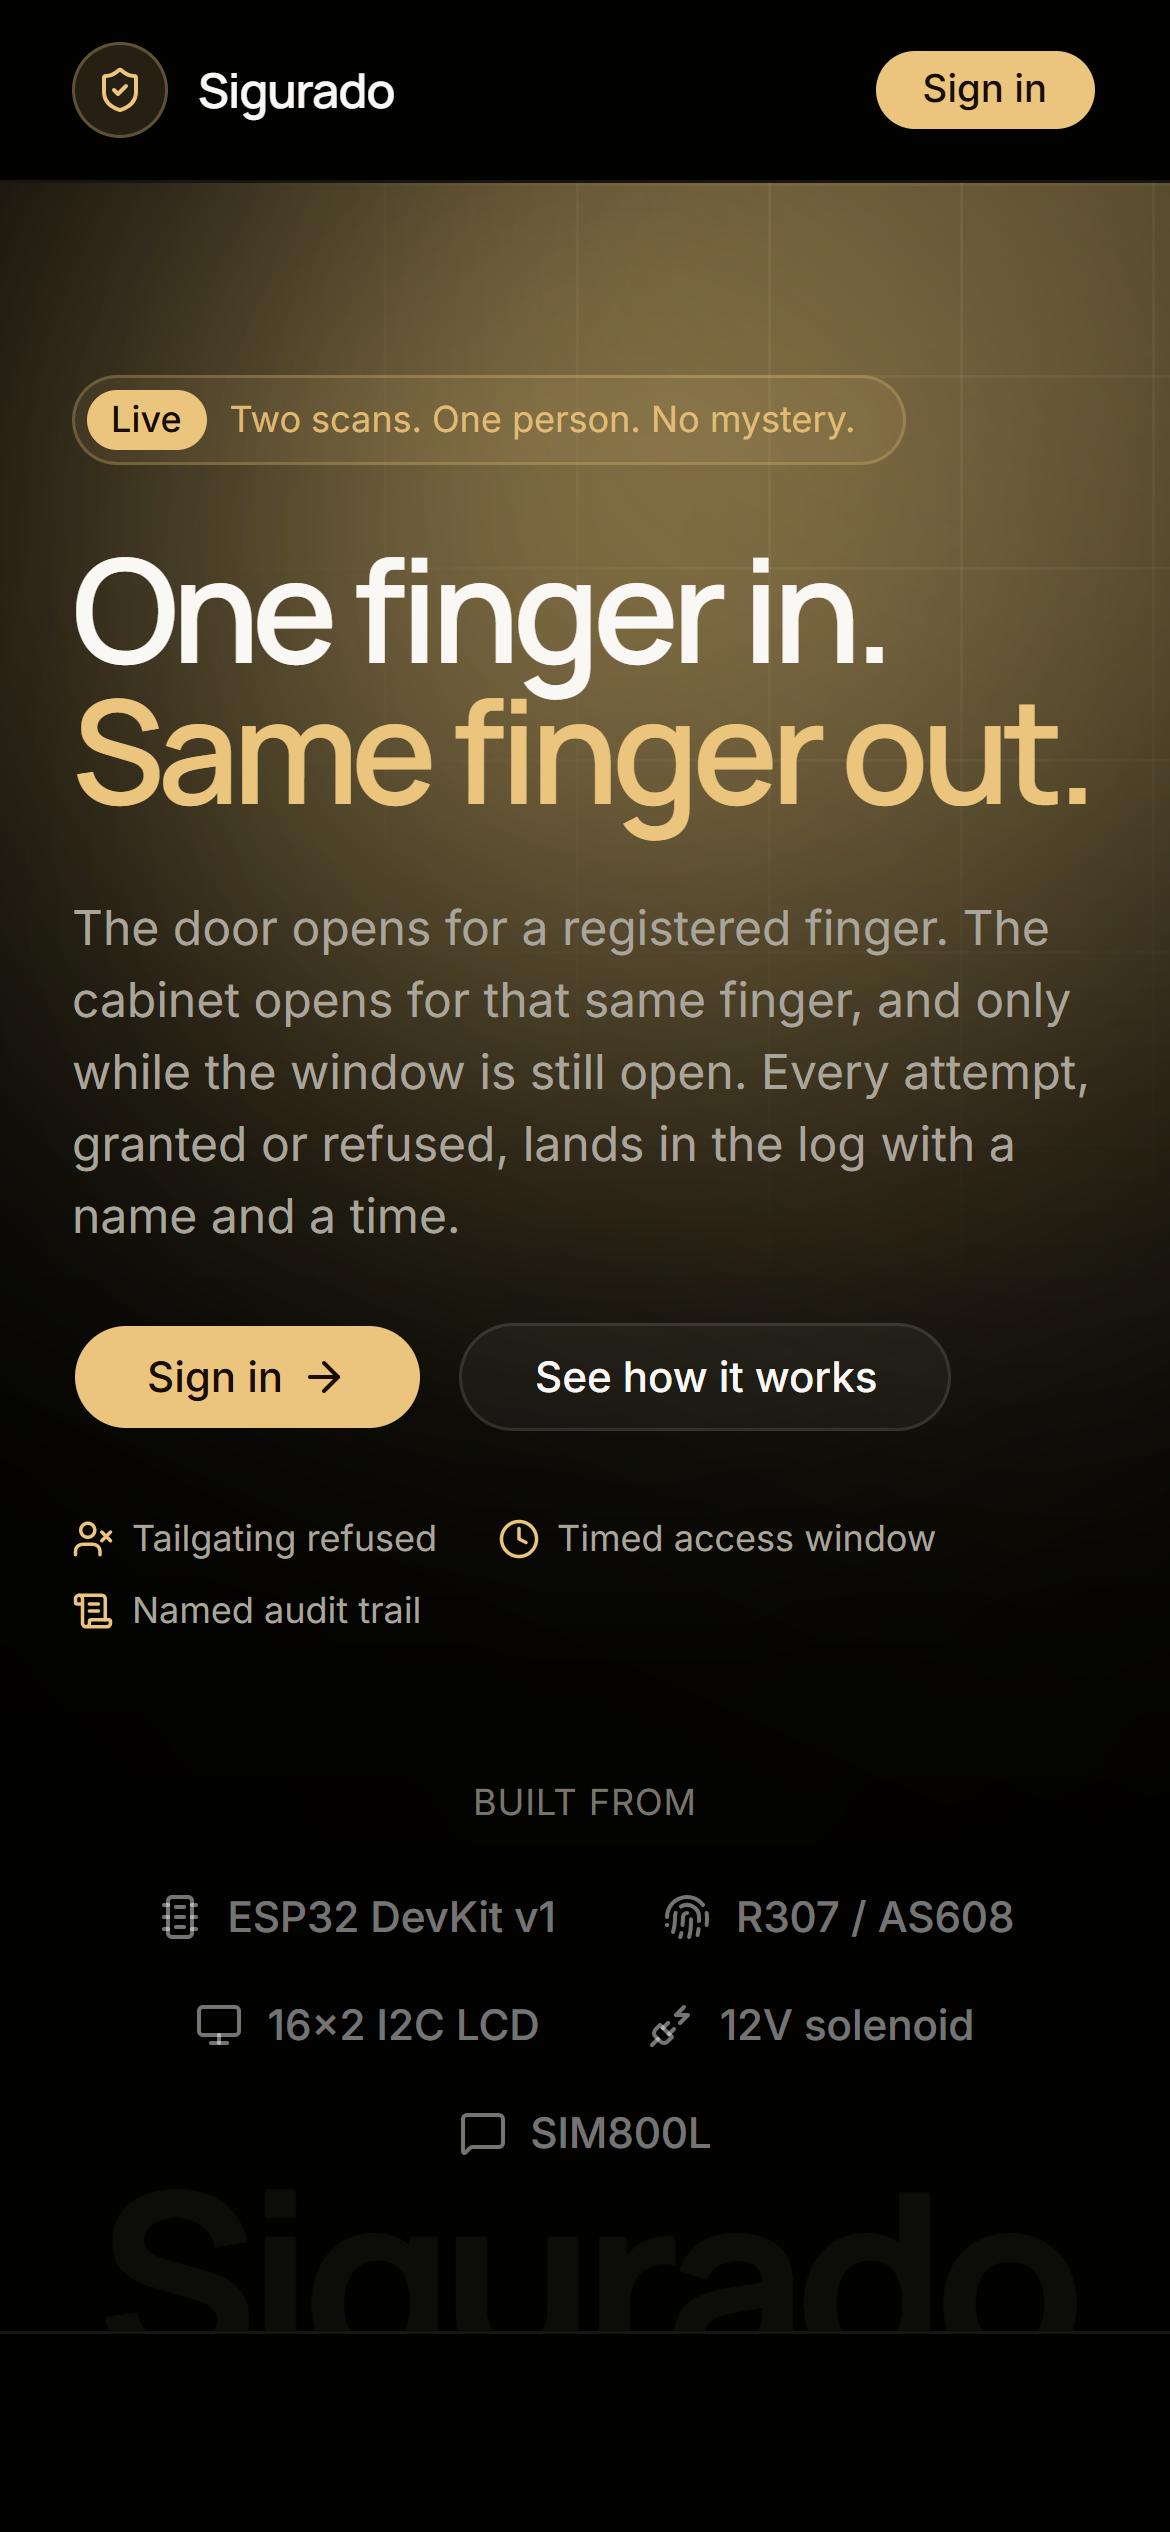
\includegraphics[width=\linewidth]{figures/mob-landing.png}
\end{minipage}\hfill
\begin{minipage}[t]{0.31\linewidth}
  \centering
  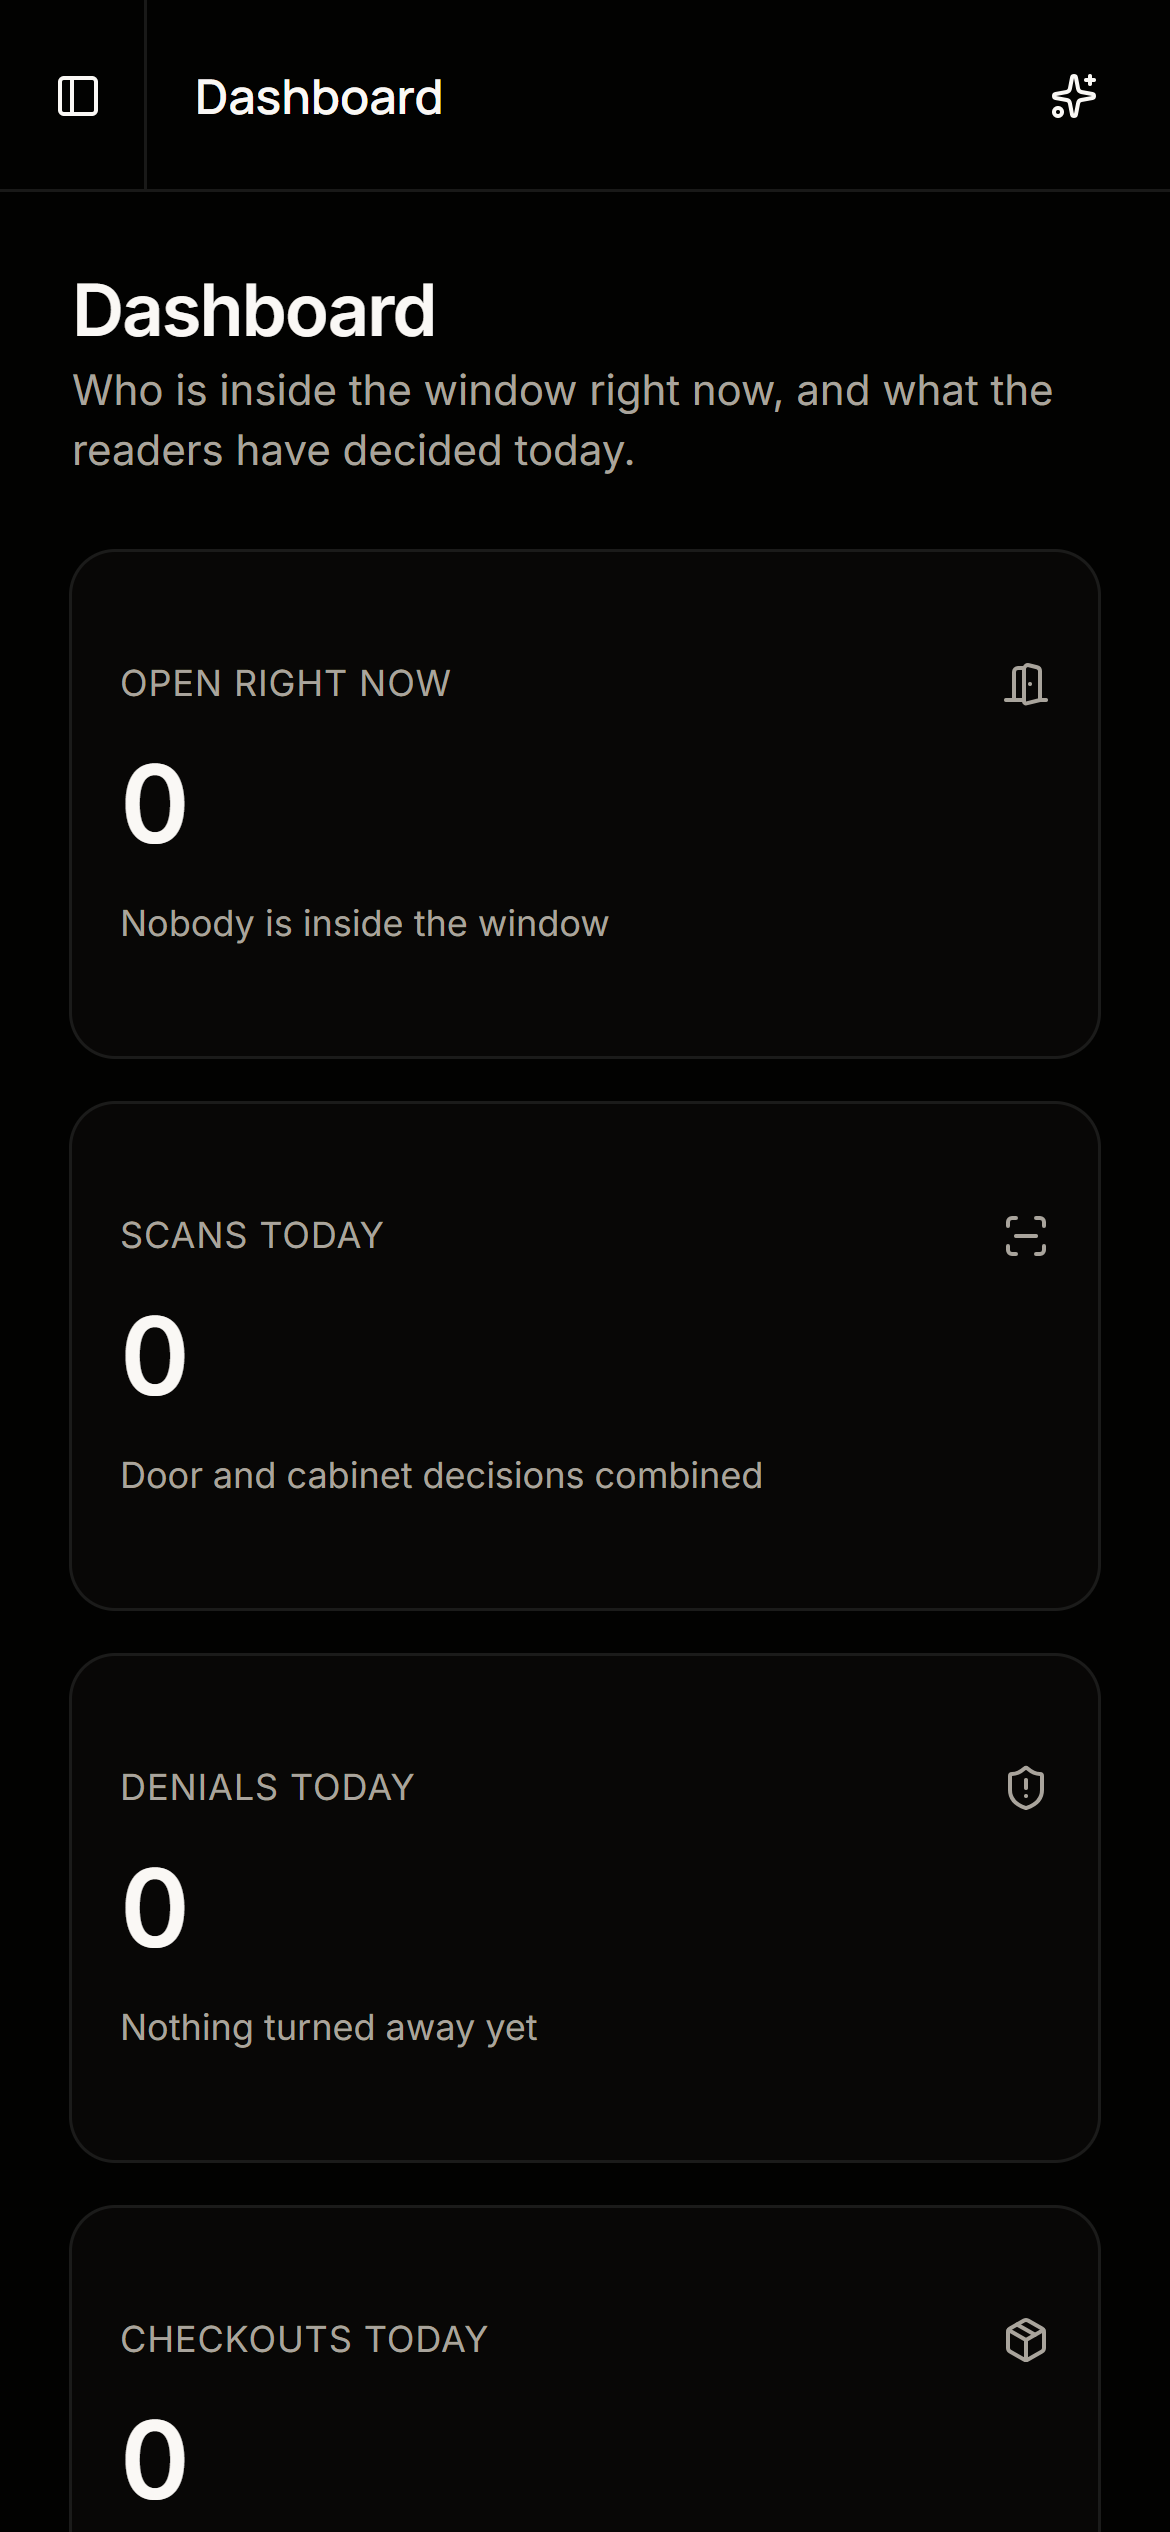
\includegraphics[width=\linewidth]{figures/mob-dashboard.png}
\end{minipage}\hfill
\begin{minipage}[t]{0.31\linewidth}
  \centering
  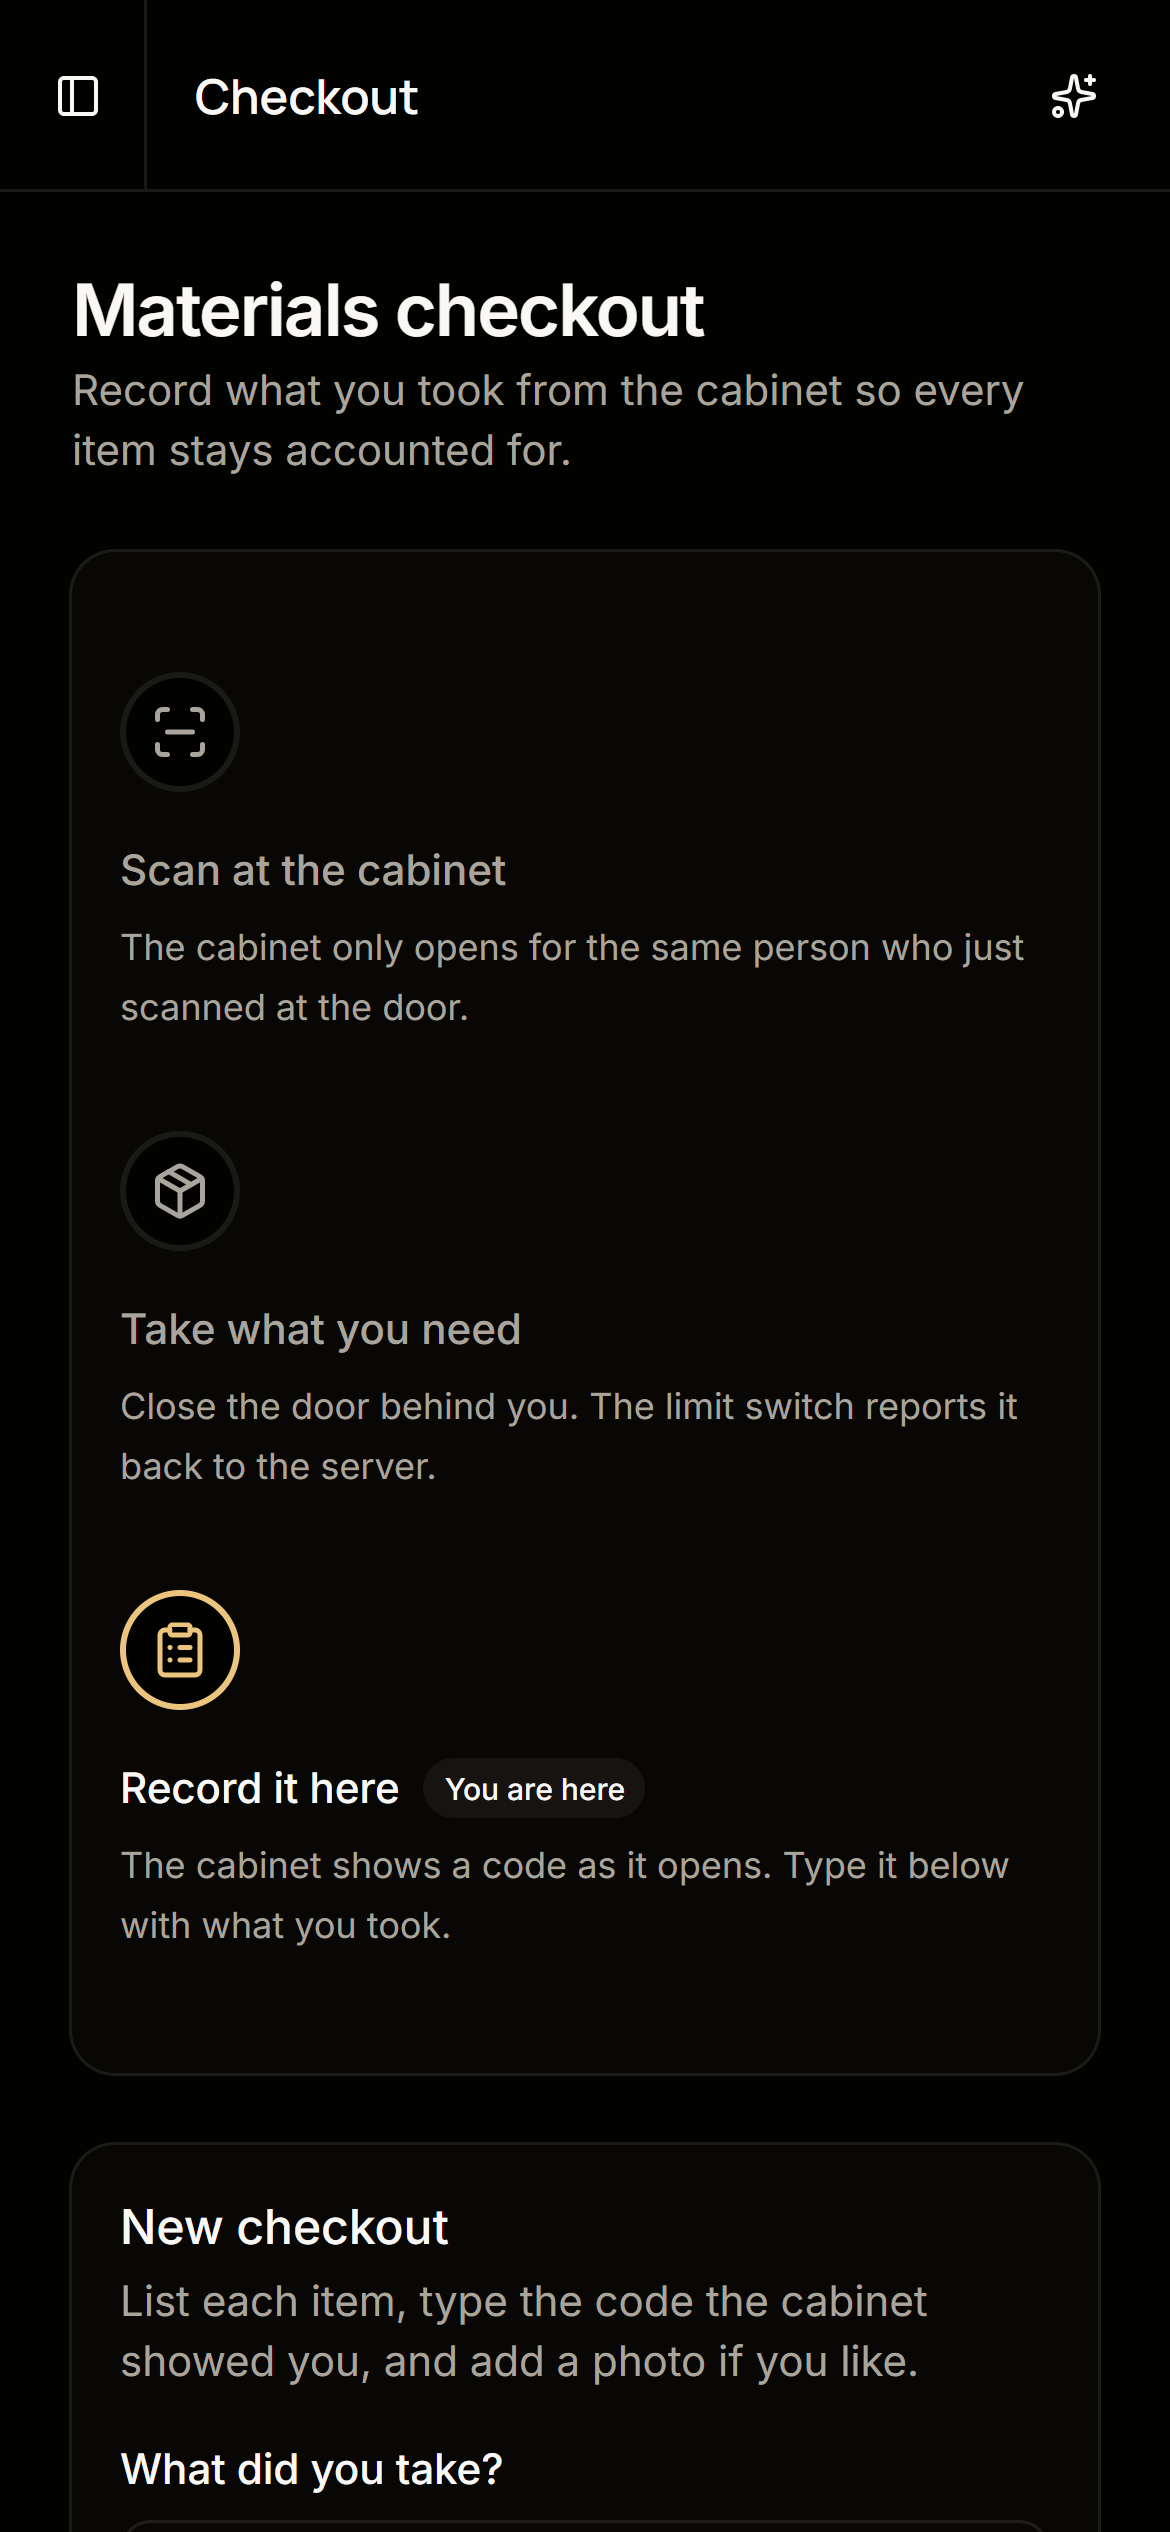
\includegraphics[width=\linewidth]{figures/mob-checkout.png}
\end{minipage}
\end{figure}

Three things change on a small screen. The side menu folds away behind a button,
so the content gets the full width. The counters stack instead of sitting in a
row. The record tables scroll sideways rather than shrinking their text, because
a column of times squeezed to four characters is worse than one the reader has
to push across.

\chapterhead{Testing and Performance}

Testing ran at three levels. Unit tests checked the decision logic on its own.
Integration tests checked that the website and the server agree with each other.
System tests exercised the assembled hardware end to end, from a finger at the
door to a borrowed item appearing in the record.

One limit applies to everything below. The tests establish that each behaviour
happens, not how fast or how reliably it happens over many attempts. Timing and
error rates were not recorded across a controlled set of trials, so the rows
marked \textbf{[MEASURE]} in Table~\ref{tab:results} and
Table~\ref{tab:timing} are left for that work.

\sectionhead{Unit and Integration Testing}

Unit testing means checking small pieces of code one at a time. We wrote 18 of
these tests for the server, where the decisions are made. They cover three
things: that passwords follow the rules, that the warning checks work on a quiet
record as well as a busy one, and that the date maths is right.

Integration testing means checking that two parts agree with each other. The
website is checked against the server automatically. That check passed with no
errors across 4{,}871 files. This catches the case where the server starts
sending something the website does not expect.

The reader firmware was compiled for the target board before flashing. Both
programs built with no errors, which confirmed that the modules link correctly
and that the libraries match the board.

\sectionhead{System Testing}

System testing means using the whole thing the way a person would. We ran the
server and the website together against a database that already held records.
This matters. An empty database returns nothing, so a fault that only appears
with real data would stay hidden.

We logged in first, on purpose. It worked and returned the right account. This
proved the system was alive, so any later failure would mean something real and
not just a dead server.

Then we opened each page the website uses. The record list, the borrow list, the
active session check, and the live feed all worked. The record list held 39
saved events of eight different kinds. All 20 pages of the website loaded.

\subsectionhead{Testing the Assembled Readers}

With both readers built and flashed, the complete sequence was exercised on the
hardware itself. A registered finger at the door released the door lock and
opened a session. The same finger at the cabinet released the cabinet within
that session. The cabinet displayed its one-time code, and the website accepted
a borrow record only when that code was entered.

The refusal paths were exercised as well, since a system that only ever grants
access has not been tested. A registered finger presented at the cabinet without
a door session first was refused, and the refusal was written to the record as a
tailgating attempt. A finger that had expired out of its session was likewise
refused. In both cases the cabinet stayed shut and the attempt appeared in the
trail with a name, a reader, and a time.

\sectionhead{Test Results}

Table~\ref{tab:results} records the outcome of every activity described above,
together with the evidence behind it. Rows marked \textbf{[MEASURE]} are
behaviours already shown to work whose performance has not yet been quantified.

\begin{table}[H]
\centering
\caption{What we tested and what happened}
\label{tab:results}
% APA permits single spacing within a table. Needed here: at double
% spacing this one runs a few points past the bottom of the page.
\linespread{1}\selectfont
\begin{tabular}{@{}p{46mm}p{26mm}p{42mm}@{}}
\toprule
What we tested & Result & How we know \\
\midrule
\multicolumn{3}{@{}l}{\textit{Software}} \\
Server unit tests      & Passed & 18 tests, none failed \\
Website and server fit & Passed & 0 errors, 4{,}871 files \\
Door reader build      & Passed & Compiled, no errors \\
Cabinet reader build   & Passed & Compiled, no errors \\
Logging in             & Passed & Correct account returned \\
Record list            & Passed & 39 events, 8 kinds \\
Borrow list            & Passed & Records returned \\
Session check          & Passed & Worked \\
Live feed              & Passed & Stayed connected \\
Website pages          & Passed & 20 of 20 loaded \\
\midrule
\multicolumn{3}{@{}l}{\textit{Assembled hardware}} \\
Door scan opens session  & Passed & Lock released, session created \\
Cabinet opens for same person & Passed & Released inside the session \\
One-time code shown      & Passed & Displayed on opening \\
Borrow record needs code & Passed & Refused without it \\
Tailgating refused       & Passed & No session, cabinet stayed shut \\
Expired session refused  & Passed & Cabinet stayed shut \\
Refusals recorded        & Passed & Written to the trail \\
\midrule
\multicolumn{3}{@{}l}{\textit{Not yet quantified}} \\
Scan time            & [MEASURE] & Works; not timed over trials \\
Unlock time          & [MEASURE] & Works; not timed over trials \\
False acceptance rate & [MEASURE] & Needs a controlled trial set \\
False rejection rate  & [MEASURE] & Needs a controlled trial set \\
Text messages        & Stand-in only & No real SIM card \\
\bottomrule
\end{tabular}
\end{table}

We found one fault, and we report it instead of quietly fixing it, because it
shows why testing with real data matters. The server sent all 39 records, but
the website showed none of them. The reason: the server had learned two new
kinds of record that the website did not know about. The website checks the
whole list at once, so one unknown item threw away all 39. The spreadsheet page,
which checks each row on its own, showed everything. That difference is what
told us where the fault was. The saved records themselves were never harmed.

\sectionhead{System Requirements}

Table~\ref{tab:reqs} states the requirements the system was designed against,
separated into what it must do and how it must behave. These are the statements
the tests above were written to check.

\begin{table}[H]
\centering
\caption{What the system must do}
\label{tab:reqs}
\linespread{1}\selectfont
\begin{tabular}{@{}p{10mm}p{100mm}@{}}
\toprule
No. & Requirement \\
\midrule
\multicolumn{2}{@{}l}{\textit{What it must do}} \\
F1 & The door opens only for a finger signed up on the door sensor. \\
F2 & A door scan starts a session for that one person, which ends by itself. \\
F3 & The cabinet opens only for the person holding a running session. \\
F4 & Every decision is saved with the person, the reader, and the time. \\
F5 & The cabinet shows a one-time code, and no borrow record is accepted
     without it. \\
F6 & The website shows which readers are working. \\
\midrule
\multicolumn{2}{@{}l}{\textit{How it must behave}} \\
N1 & Readers never decide on their own. \\
N2 & Fingerprints never leave the sensor. \\
N3 & Nobody can edit or delete a saved reader record, not even an
     administrator. \\
N4 & Each reader has its own password, which can be changed on its own. \\
N5 & The program must fit in the chip with room to spare. \\
N6 & The reader must never freeze while the lock is open or a message is
     showing. \\
\bottomrule
\end{tabular}
\end{table}

Every requirement in the table was exercised during testing. F1 to F6 were
demonstrated on the assembled readers, as recorded in
Table~\ref{tab:results}. N1, N2 and N4 follow from how the system is built and
were confirmed by inspection: a reader holds no decision logic, no template
leaves the sensor, and each reader carries its own credentials. N3 was confirmed
by attempting to edit a reader record through the interface, which offers no
route to do so. N5 is measured below. N6 was observed on the hardware, where a
second finger could be presented while a message was still on screen.

\sectionhead{Performance Analysis}

Performance is examined here in two ways. The first is what the finished program
demands of the chip, which the build reports exactly. The second is how the
design sits against systems that have already been measured and published.

\subsectionhead{Use of Chip Resources}

Our program fills about 81 percent of its 1.2 MB space. That meets requirement
N5, but only just. Adding features later will be limited by this, not by speed
or memory.

RAM is not a problem, and the reason is a design choice. Fingerprints stay in
the sensor, so the biggest piece of data never reaches our chip. That turns the
usual tightest limit on this kind of project into a non-issue. It also answers
the small-memory warning raised by \textcite{rahman2026}.

Speed is not a problem either. \textcite{espressif2025} rate the chip at 1079.96
CoreMark, a standard speed score. Our reader only waits on a slow sensor, builds
a short message, and keeps Wi-Fi alive. Two processors mean the Wi-Fi keeps
running while the sensor is read.

\subsectionhead{Timing}

Table~\ref{tab:timing} separates the intervals fixed by the design, which are
known exactly, from those that depend on the sensor and the network and would
have to be timed over repeated trials.

\begin{table}[H]
\centering
\caption{Timings we set, and timings still to be measured}
\label{tab:timing}
\begin{tabular}{@{}p{42mm}p{26mm}p{42mm}@{}}
\toprule
Interval & Value & Status \\
\midrule
Session length        & 120~s     & Set in the server \\
Checkout code lifetime & 900~s    & Set in the server \\
Enrollment code lifetime & 300~s  & Set in the server \\
Door lock stays open  & 3~s       & Set in the reader \\
Cabinet lock stays open & 4~s     & Set in the reader \\
Message on screen     & 2.5~s     & Set in the reader \\
``Still here'' signal & 30~s      & Set in the reader \\
Scan time             & [MEASURE] & Observed to work; not timed \\
Unlock time           & [MEASURE] & Observed to work; not timed \\
\bottomrule
\end{tabular}
\end{table}

\subsectionhead{Comparison With Published Systems}

The figures below belong to other people's systems. They are the benchmarks
this system should be compared against once its own numbers are recorded.

\textcite{alsayaydeh2025} measured a scan at about one second and an unlock at
five seconds on a setup much like ours. They admitted the wrong person 1.32
percent of the time and turned away the right person 26.32 percent of the time.
The second figure is the warning. A system that rejects one honest person in
four will end up propped open, and a propped door defeats everything behind it.

\textcite{mohammed2025} report a mean authentication time of 235 milliseconds
and a 68 percent drop in fraudulent access. Their timing is not a fair
comparison, since their pipeline runs on server-class machines rather than a
microcontroller. The 68 percent is the relevant figure: it is the scale of
improvement that checking twice is expected to deliver, and the effect the
door-to-cabinet sequence is built to reproduce.

Two properties of this system have no counterpart in either study. Refusals are
recorded as carefully as approvals, so tailgating attempts become a countable
quantity rather than an assumption, and the refusal tests above confirm those
records are written. Reader events are also append-only by construction, which
is the accountability property \textcite{koisser2023} argue a record must have
before it can be used as evidence.

\chapterhead{Conclusion}

\sectionhead{Problems Encountered}

Six problems shaped the final design. The first three appeared in the software, where they were found and corrected. The next two were electrical, and were caught while the readers were being assembled. The last belongs to the room itself.

\subsectionhead{Slot Numbers Meant Different People}

Each sensor keeps its own list of fingerprints. Slot 7 on the door sensor and
slot 7 on the cabinet sensor are two different people. Our first design treated
slot 7 as one person everywhere. That would have opened the cabinet for the
wrong person, and the record would have looked perfectly normal.

\subsectionhead{A Reader Cannot Be Trusted to Decide}

At first each reader decided by itself and then told the server. That is easy to
build and wrong. A reader hangs on a wall. Anyone can open it and copy or fake
its messages. Anything that decides who gets in has to be decided by the server.

\subsectionhead{One Unknown Record Emptied the Whole Page}

Described in Chapter 3. The server learned two new kinds of record. The website
did not know them, so it threw away all 39 records instead of just the two. The
page looked empty, and no error was shown.

\subsectionhead{Settings Were Cut Without Warning}

The server reads its settings from a text file. That file quietly cuts anything
after a space. A name with a space in it gets shortened, and nothing tells you.

\subsectionhead{Electrical Problems That Only Appear in Hardware}

Three problems surfaced while the readers were being wired up. The lock
pulls a lot of current when it opens and will restart the chip if the two
share one supply. The text unit does the same when it sends. And one of its
wires cannot take the chip's full signal strength. Each of these shows up as
a random restart, which is hard to trace back to its cause.

\subsectionhead{The Door Reader May Not Reach the Wi-Fi}

The door is the farthest point from the router. A reader that cannot reach the
server cannot ask permission, and by design it will not decide alone. So it
opens nothing.

\sectionhead{Troubleshooting}

This section describes how the problems above were traced. In each case the useful part was not the fix but the observation that made the fault visible in the first place.

\subsectionhead{Finding the Empty Page Fault}

The server replied correctly with a full page of data, so the server and the
network were ruled out at once. The clue was that the spreadsheet page showed
all 39 records while the record page showed none. Both read the same data, so
the difference had to be in how each one read it. Comparing the kinds of record
in the data against the kinds the website accepted found the two unknown ones.

The wider lesson is what made it visible at all: we tested with real data. With
an empty database both pages show nothing, and the fault would have looked like
normal behaviour.

\subsectionhead{Always Start With Something That Works}

Every round of testing began with a request we knew should succeed. Without
that, a test where everything fails only proves the server is off. It says
nothing about the parts being tested.

\subsectionhead{Checking Code Before Flashing}

Before the boards were flashed, the only available checks were the ones the
tools can make: that the code compiles, that the modules link, and that the
image fits the chip with measurable room left. Those checks caught real
mistakes early, but they cannot show behaviour. Everything about how the
system actually behaves came afterwards, from the assembled readers.

\sectionhead{Solutions and Conclusions}

This section sets out what was changed in response to those problems, what the study achieved, and what it was not able to show.

\subsectionhead{What We Fixed}

Finger records now carry the name of the reader they came from, so a slot number
can never be matched against the wrong sensor. The cost is that people sign up
twice, once at each reader. We accepted that cost rather than hide it.

All decisions moved to the server. Readers log in with their own ID and
password, not a person's, so a stolen reader gives away only itself. Reader
records were made permanent, with no way to edit or delete them for anyone,
including administrators. A wrong record is corrected by adding a right one.

The electrical problems were solved in the wiring. The lock and the text unit
each got their own power supply, sharing only a ground wire with the chip, and
the text unit's weak wire got a voltage reducer. Where the door reader cannot
reach the Wi-Fi, the cabinet reader can share its connection.

The empty page fault is still open. The fix is to teach the website all the
kinds of record the server sends, and to check each row on its own so one
unknown item cannot throw away a whole page.

\subsectionhead{Conclusion}

This project set out to prove who took materials from a school stockroom, and to
record it so nobody can change it afterwards.

The design goals were met. We documented how the chip's processors, memory,
pins, and Wi-Fi work, and showed that each one shaped a real decision. The
clearest example is memory. By leaving fingerprints in the sensor, the largest
piece of data never reaches the chip. What is usually the tightest limit on this
kind of project stopped being a limit at all.

The software goals were met and tested. The two-step check, the session, the
permanent record, and the code-locked borrow list all work, and Chapter 3 shows
the results. Safety comes from the shape of the design, not from one clever
part. Decisions sit in one place, readers can only speak as themselves, and
refusals are saved as carefully as approvals.

The main goal was demonstrated. Both readers were built, flashed, and run
through the full sequence. The cabinet refused a finger that held no door
session, and the attempt was written to the record. What remains is measurement
rather than function. Until scan time, unlock time, and error rates are recorded
over repeated trials, this system cannot be set beside the figures reported by
\textcite{alsayaydeh2025}, and the 68 percent reduction that
\textcite{mohammed2025} measured cannot be confirmed in this setting.

Two limits remain even now that the hardware is built. The sensor does the
matching, so we inherit its accuracy and have no way to spot a fake finger; the
seaweed-jelly fakes shown by \textcite{rad2024} would get through. And the
borrow list is still typed by a person. We can prove the cabinet opened and who
opened it, but not that the typed list is complete. Closing that gap would mean
sensing the items themselves, which is a different project.

\subsectionhead{Recommendations}

The following work would close the gaps this study leaves open. The first item matters most, because it is the difference between a system shown to work and a system whose performance is known.

\begin{enumerate}
  \item Record scan time, unlock time, and error rates over a controlled set
        of trials, so the system can be compared against published figures.
  \item Fix the empty page fault before the system is used for real.
  \item Test with a real SIM card and a real phone network.
  \item Consider a sensor with fake-finger detection, given the weakness shown
        by \textcite{rad2024}.
  \item Watch the refusal count once the system runs. It shows how often
        tailgating is actually tried.
\end{enumerate}


\printbibliography

\end{document}
